\documentclass[]{article}
\usepackage{lmodern}
\usepackage{amssymb,amsmath}
\usepackage{ifxetex,ifluatex}
\usepackage{fixltx2e} % provides \textsubscript
\ifnum 0\ifxetex 1\fi\ifluatex 1\fi=0 % if pdftex
  \usepackage[T1]{fontenc}
  \usepackage[utf8]{inputenc}
\else % if luatex or xelatex
  \ifxetex
    \usepackage{mathspec}
  \else
    \usepackage{fontspec}
  \fi
  \defaultfontfeatures{Ligatures=TeX,Scale=MatchLowercase}
\fi
% use upquote if available, for straight quotes in verbatim environments
\IfFileExists{upquote.sty}{\usepackage{upquote}}{}
% use microtype if available
\IfFileExists{microtype.sty}{%
\usepackage{microtype}
\UseMicrotypeSet[protrusion]{basicmath} % disable protrusion for tt fonts
}{}
\usepackage[margin=1in]{geometry}
\usepackage{hyperref}
\hypersetup{unicode=true,
            pdftitle={Single studies using the CohortMethod package},
            pdfauthor={Martijn J. Schuemie, Marc A. Suchard and Patrick Ryan},
            pdfborder={0 0 0},
            breaklinks=true}
\urlstyle{same}  % don't use monospace font for urls
\usepackage{color}
\usepackage{fancyvrb}
\newcommand{\VerbBar}{|}
\newcommand{\VERB}{\Verb[commandchars=\\\{\}]}
\DefineVerbatimEnvironment{Highlighting}{Verbatim}{commandchars=\\\{\}}
% Add ',fontsize=\small' for more characters per line
\usepackage{framed}
\definecolor{shadecolor}{RGB}{248,248,248}
\newenvironment{Shaded}{\begin{snugshade}}{\end{snugshade}}
\newcommand{\AlertTok}[1]{\textcolor[rgb]{0.94,0.16,0.16}{#1}}
\newcommand{\AnnotationTok}[1]{\textcolor[rgb]{0.56,0.35,0.01}{\textbf{\textit{#1}}}}
\newcommand{\AttributeTok}[1]{\textcolor[rgb]{0.77,0.63,0.00}{#1}}
\newcommand{\BaseNTok}[1]{\textcolor[rgb]{0.00,0.00,0.81}{#1}}
\newcommand{\BuiltInTok}[1]{#1}
\newcommand{\CharTok}[1]{\textcolor[rgb]{0.31,0.60,0.02}{#1}}
\newcommand{\CommentTok}[1]{\textcolor[rgb]{0.56,0.35,0.01}{\textit{#1}}}
\newcommand{\CommentVarTok}[1]{\textcolor[rgb]{0.56,0.35,0.01}{\textbf{\textit{#1}}}}
\newcommand{\ConstantTok}[1]{\textcolor[rgb]{0.00,0.00,0.00}{#1}}
\newcommand{\ControlFlowTok}[1]{\textcolor[rgb]{0.13,0.29,0.53}{\textbf{#1}}}
\newcommand{\DataTypeTok}[1]{\textcolor[rgb]{0.13,0.29,0.53}{#1}}
\newcommand{\DecValTok}[1]{\textcolor[rgb]{0.00,0.00,0.81}{#1}}
\newcommand{\DocumentationTok}[1]{\textcolor[rgb]{0.56,0.35,0.01}{\textbf{\textit{#1}}}}
\newcommand{\ErrorTok}[1]{\textcolor[rgb]{0.64,0.00,0.00}{\textbf{#1}}}
\newcommand{\ExtensionTok}[1]{#1}
\newcommand{\FloatTok}[1]{\textcolor[rgb]{0.00,0.00,0.81}{#1}}
\newcommand{\FunctionTok}[1]{\textcolor[rgb]{0.00,0.00,0.00}{#1}}
\newcommand{\ImportTok}[1]{#1}
\newcommand{\InformationTok}[1]{\textcolor[rgb]{0.56,0.35,0.01}{\textbf{\textit{#1}}}}
\newcommand{\KeywordTok}[1]{\textcolor[rgb]{0.13,0.29,0.53}{\textbf{#1}}}
\newcommand{\NormalTok}[1]{#1}
\newcommand{\OperatorTok}[1]{\textcolor[rgb]{0.81,0.36,0.00}{\textbf{#1}}}
\newcommand{\OtherTok}[1]{\textcolor[rgb]{0.56,0.35,0.01}{#1}}
\newcommand{\PreprocessorTok}[1]{\textcolor[rgb]{0.56,0.35,0.01}{\textit{#1}}}
\newcommand{\RegionMarkerTok}[1]{#1}
\newcommand{\SpecialCharTok}[1]{\textcolor[rgb]{0.00,0.00,0.00}{#1}}
\newcommand{\SpecialStringTok}[1]{\textcolor[rgb]{0.31,0.60,0.02}{#1}}
\newcommand{\StringTok}[1]{\textcolor[rgb]{0.31,0.60,0.02}{#1}}
\newcommand{\VariableTok}[1]{\textcolor[rgb]{0.00,0.00,0.00}{#1}}
\newcommand{\VerbatimStringTok}[1]{\textcolor[rgb]{0.31,0.60,0.02}{#1}}
\newcommand{\WarningTok}[1]{\textcolor[rgb]{0.56,0.35,0.01}{\textbf{\textit{#1}}}}
\usepackage{graphicx,grffile}
\makeatletter
\def\maxwidth{\ifdim\Gin@nat@width>\linewidth\linewidth\else\Gin@nat@width\fi}
\def\maxheight{\ifdim\Gin@nat@height>\textheight\textheight\else\Gin@nat@height\fi}
\makeatother
% Scale images if necessary, so that they will not overflow the page
% margins by default, and it is still possible to overwrite the defaults
% using explicit options in \includegraphics[width, height, ...]{}
\setkeys{Gin}{width=\maxwidth,height=\maxheight,keepaspectratio}
\IfFileExists{parskip.sty}{%
\usepackage{parskip}
}{% else
\setlength{\parindent}{0pt}
\setlength{\parskip}{6pt plus 2pt minus 1pt}
}
\setlength{\emergencystretch}{3em}  % prevent overfull lines
\providecommand{\tightlist}{%
  \setlength{\itemsep}{0pt}\setlength{\parskip}{0pt}}
\setcounter{secnumdepth}{5}
% Redefines (sub)paragraphs to behave more like sections
\ifx\paragraph\undefined\else
\let\oldparagraph\paragraph
\renewcommand{\paragraph}[1]{\oldparagraph{#1}\mbox{}}
\fi
\ifx\subparagraph\undefined\else
\let\oldsubparagraph\subparagraph
\renewcommand{\subparagraph}[1]{\oldsubparagraph{#1}\mbox{}}
\fi

%%% Use protect on footnotes to avoid problems with footnotes in titles
\let\rmarkdownfootnote\footnote%
\def\footnote{\protect\rmarkdownfootnote}

%%% Change title format to be more compact
\usepackage{titling}

% Create subtitle command for use in maketitle
\newcommand{\subtitle}[1]{
  \posttitle{
    \begin{center}\large#1\end{center}
    }
}

\setlength{\droptitle}{-2em}
  \title{Single studies using the CohortMethod package}
  \pretitle{\vspace{\droptitle}\centering\huge}
  \posttitle{\par}
  \author{Martijn J. Schuemie, Marc A. Suchard and Patrick Ryan}
  \preauthor{\centering\large\emph}
  \postauthor{\par}
  \predate{\centering\large\emph}
  \postdate{\par}
  \date{2018-06-14}


\begin{document}
\maketitle

{
\setcounter{tocdepth}{2}
\tableofcontents
}
\hypertarget{introduction}{%
\section{Introduction}\label{introduction}}

This vignette describes how you can use the \texttt{CohortMethod}
package to perform a single new-user cohort study. We will walk through
all the steps needed to perform an exemplar study, and we have selected
the well-studied topic of the effect of coxibs versus non-selective
non-steroidal anti-inflammatory drugs (NSAIDs) on gastrointestinal (GI)
bleeding-related hospitalization. For simplicity, we focus on one coxib
-- celecoxib -- and one non-selective NSAID -- diclofenac.

\hypertarget{installation-instructions}{%
\section{Installation instructions}\label{installation-instructions}}

Before installing the \texttt{CohortMethod} package make sure you have
Java available. Java can be downloaded from
\href{http://www.java.com}{www.java.com}. For Windows users, RTools is
also necessary. RTools can be downloaded from
\href{http://cran.r-project.org/bin/windows/Rtools/}{CRAN}.

The \texttt{CohortMethod} package is currently maintained in a
\href{https://github.com/OHDSI/CohortMethod}{Github repository}, and has
dependencies on other packages in Github. All of these packages can be
downloaded and installed from within R using the \texttt{drat} package:

\begin{Shaded}
\begin{Highlighting}[]
\KeywordTok{install.packages}\NormalTok{(}\StringTok{"drat"}\NormalTok{)}
\NormalTok{drat}\OperatorTok{::}\KeywordTok{addRepo}\NormalTok{(}\StringTok{"OHDSI"}\NormalTok{)}
\KeywordTok{install.packages}\NormalTok{(}\StringTok{"CohortMethod"}\NormalTok{)}
\end{Highlighting}
\end{Shaded}

Once installed, you can type \texttt{library(CohortMethod)} to load the
package.

\hypertarget{data-extraction}{%
\section{Data extraction}\label{data-extraction}}

The first step in running the \texttt{CohortMethod} is extracting all
necessary data from the database server holding the data in the
Observational Medical Outcomes Partnership (OMOP) Common Data Model
(CDM) format.

\hypertarget{configuring-the-connection-to-the-server}{%
\subsection{Configuring the connection to the
server}\label{configuring-the-connection-to-the-server}}

We need to tell R how to connect to the server where the data are.
\texttt{CohortMethod} uses the \texttt{DatabaseConnector} package, which
provides the \texttt{createConnectionDetails} function. Type
\texttt{?createConnectionDetails} for the specific settings required for
the various database management systems (DBMS). For example, one might
connect to a PostgreSQL database using this code:

\begin{Shaded}
\begin{Highlighting}[]
\NormalTok{connectionDetails <-}\StringTok{ }\KeywordTok{createConnectionDetails}\NormalTok{(}\DataTypeTok{dbms =} \StringTok{"postgresql"}\NormalTok{,}
                                             \DataTypeTok{server =} \StringTok{"localhost/ohdsi"}\NormalTok{,}
                                             \DataTypeTok{user =} \StringTok{"joe"}\NormalTok{,}
                                             \DataTypeTok{password =} \StringTok{"supersecret"}\NormalTok{)}

\NormalTok{cdmDatabaseSchema <-}\StringTok{ "my_cdm_data"}
\NormalTok{resultsDatabaseSchema <-}\StringTok{ "my_results"}
\end{Highlighting}
\end{Shaded}

The last two lines define the \texttt{cdmDatabaseSchema} and
\texttt{resultSchema} variables. We'll use these later to tell R where
the data in CDM format live, and where we want to write intermediate
tables. Note that for Microsoft SQL Server, databaseschemas need to
specify both the database and the schema, so for example
\texttt{cdmDatabaseSchema\ \textless{}-\ "my\_cdm\_data.dbo"}.

\hypertarget{preparing-the-exposures-and-outcomes}{%
\subsection{Preparing the exposures and
outcome(s)}\label{preparing-the-exposures-and-outcomes}}

We need to define the exposures and outcomes for our study. One could
use an external cohort definition tools, but in this example we do this
by writing SQL statements against the OMOP CDM that populate a table of
events in which we are interested. The resulting table should have the
same structure as the \texttt{cohort} table in the CDM. This means it
should have the fields \texttt{cohort\_definition\_id},
\texttt{cohort\_start\_date}, \texttt{cohort\_end\_date},and
\texttt{subject\_id}.

For our example study, we have created a file called
\emph{coxibVsNonselVsGiBleed.sql} with the following contents:

\begin{Shaded}
\begin{Highlighting}[]
\CommentTok{/***********************************}
\CommentTok{File coxibVsNonselVsGiBleed.sql}
\CommentTok{***********************************/}

\KeywordTok{IF}\NormalTok{ OBJECT_ID(}\StringTok{'@resultsDatabaseSchema.coxibVsNonselVsGiBleed'}\NormalTok{, }\StringTok{'U'}\NormalTok{) }\KeywordTok{IS} \KeywordTok{NOT} \KeywordTok{NULL}
  \KeywordTok{DROP} \KeywordTok{TABLE}\NormalTok{ @resultsDatabaseSchema.coxibVsNonselVsGiBleed;}

\KeywordTok{CREATE} \KeywordTok{TABLE}\NormalTok{ @resultsDatabaseSchema.coxibVsNonselVsGiBleed (}
\NormalTok{  cohort_definition_id }\DataTypeTok{INT}\NormalTok{,}
\NormalTok{  cohort_start_date }\DataTypeTok{DATE}\NormalTok{,}
\NormalTok{    cohort_end_date }\DataTypeTok{DATE}\NormalTok{,}
\NormalTok{    subject_id BIGINT}
\NormalTok{    );}

\KeywordTok{INSERT} \KeywordTok{INTO}\NormalTok{ @resultsDatabaseSchema.coxibVsNonselVsGiBleed (}
\NormalTok{    cohort_definition_id,}
\NormalTok{    cohort_start_date,}
\NormalTok{    cohort_end_date,}
\NormalTok{    subject_id}
\NormalTok{    )}
\KeywordTok{SELECT} \DecValTok{1}\NormalTok{, }\CommentTok{-- Exposure}
\NormalTok{    drug_era_start_date,}
\NormalTok{    drug_era_end_date,}
\NormalTok{    person_id}
\KeywordTok{FROM}\NormalTok{ @cdmDatabaseSchema.drug_era}
\KeywordTok{WHERE}\NormalTok{ drug_concept_id = }\DecValTok{1118084}\NormalTok{;}\CommentTok{-- celecoxib}

\KeywordTok{INSERT} \KeywordTok{INTO}\NormalTok{ @resultsDatabaseSchema.coxibVsNonselVsGiBleed (}
\NormalTok{    cohort_definition_id,}
\NormalTok{    cohort_start_date,}
\NormalTok{    cohort_end_date,}
\NormalTok{    subject_id}
\NormalTok{    )}
\KeywordTok{SELECT} \DecValTok{2}\NormalTok{, }\CommentTok{-- Comparator}
\NormalTok{    drug_era_start_date,}
\NormalTok{    drug_era_end_date,}
\NormalTok{    person_id}
\KeywordTok{FROM}\NormalTok{ @cdmDatabaseSchema.drug_era}
\KeywordTok{WHERE}\NormalTok{ drug_concept_id = }\DecValTok{1124300}\NormalTok{; }\CommentTok{--diclofenac}

\KeywordTok{INSERT} \KeywordTok{INTO}\NormalTok{ @resultsDatabaseSchema.coxibVsNonselVsGiBleed (}
\NormalTok{    cohort_definition_id,}
\NormalTok{    cohort_start_date,}
\NormalTok{    cohort_end_date,}
\NormalTok{    subject_id}
\NormalTok{    )}
\KeywordTok{SELECT} \DecValTok{3}\NormalTok{, }\CommentTok{-- Outcome}
\NormalTok{    condition_start_date,}
\NormalTok{    condition_end_date,}
\NormalTok{    condition_occurrence.person_id}
\KeywordTok{FROM}\NormalTok{ @cdmDatabaseSchema.condition_occurrence}
\KeywordTok{INNER} \KeywordTok{JOIN}\NormalTok{ @cdmDatabaseSchema.visit_occurrence}
    \KeywordTok{ON}\NormalTok{ condition_occurrence.visit_occurrence_id = visit_occurrence.visit_occurrence_id}
\KeywordTok{WHERE}\NormalTok{ condition_concept_id }\KeywordTok{IN}\NormalTok{ (}
        \KeywordTok{SELECT}\NormalTok{ descendant_concept_id}
        \KeywordTok{FROM}\NormalTok{ @cdmDatabaseSchema.concept_ancestor}
        \KeywordTok{WHERE}\NormalTok{ ancestor_concept_id = }\DecValTok{192671} \CommentTok{-- GI - Gastrointestinal haemorrhage}
\NormalTok{        )}
    \KeywordTok{AND}\NormalTok{ visit_occurrence.visit_concept_id }\KeywordTok{IN}\NormalTok{ (}\DecValTok{9201}\NormalTok{, }\DecValTok{9203}\NormalTok{);}
\end{Highlighting}
\end{Shaded}

This is parameterized SQL which can be used by the \texttt{SqlRender}
package. We use parameterized SQL so we do not have to pre-specify the
names of the CDM and result schemas. That way, if we want to run the SQL
on a different schema, we only need to change the parameter values; we
do not have to change the SQL code. By also making use of translation
functionality in \texttt{SqlRender}, we can make sure the SQL code can
be run in many different environments.

\begin{Shaded}
\begin{Highlighting}[]
\KeywordTok{library}\NormalTok{(SqlRender)}
\NormalTok{sql <-}\StringTok{ }\KeywordTok{readSql}\NormalTok{(}\StringTok{"coxibVsNonselVsGiBleed.sql"}\NormalTok{)}
\NormalTok{sql <-}\StringTok{ }\KeywordTok{renderSql}\NormalTok{(sql,}
                 \DataTypeTok{cdmDatabaseSchema =}\NormalTok{ cdmDatabaseSchema,}
                 \DataTypeTok{resultsDatabaseSchema =}\NormalTok{ resultsDatabaseSchema)}\OperatorTok{$}\NormalTok{sql}
\NormalTok{sql <-}\StringTok{ }\KeywordTok{translateSql}\NormalTok{(sql, }\DataTypeTok{targetDialect =}\NormalTok{ connectionDetails}\OperatorTok{$}\NormalTok{dbms)}\OperatorTok{$}\NormalTok{sql}

\NormalTok{connection <-}\StringTok{ }\KeywordTok{connect}\NormalTok{(connectionDetails)}
\KeywordTok{executeSql}\NormalTok{(connection, sql)}
\end{Highlighting}
\end{Shaded}

In this code, we first read the SQL from the file into memory. In the
next line, we replace the two parameter names with the actual values. We
then translate the SQL into the dialect appropriate for the DBMS we
already specified in the \texttt{connectionDetails}. Next, we connect to
the server, and submit the rendered and translated SQL.

If all went well, we now have a table with the events of interest. We
can see how many events per type:

\begin{Shaded}
\begin{Highlighting}[]
\NormalTok{sql <-}\StringTok{ }\KeywordTok{paste}\NormalTok{(}\StringTok{"SELECT cohort_definition_id, COUNT(*) AS count"}\NormalTok{,}
             \StringTok{"FROM @resultsDatabaseSchema.coxibVsNonselVsGiBleed"}\NormalTok{,}
             \StringTok{"GROUP BY cohort_definition_id"}\NormalTok{)}
\NormalTok{sql <-}\StringTok{ }\KeywordTok{renderSql}\NormalTok{(sql, }\DataTypeTok{resultsDatabaseSchema =}\NormalTok{ resultsDatabaseSchema)}\OperatorTok{$}\NormalTok{sql}
\NormalTok{sql <-}\StringTok{ }\KeywordTok{translateSql}\NormalTok{(sql, }\DataTypeTok{targetDialect =}\NormalTok{ connectionDetails}\OperatorTok{$}\NormalTok{dbms)}\OperatorTok{$}\NormalTok{sql}

\KeywordTok{querySql}\NormalTok{(connection, sql)}
\end{Highlighting}
\end{Shaded}

\begin{verbatim}
#>   cohort_concept_id  count
#> 1                 1 184979
#> 2                 2 798752
#> 3                 3 635619
\end{verbatim}

\hypertarget{extracting-the-data-from-the-server}{%
\subsection{Extracting the data from the
server}\label{extracting-the-data-from-the-server}}

Now we can tell \texttt{CohortMethod} to define the cohorts based on our
events, construct covariates, and extract all necessary data for our
analysis.

\textbf{Important}: The target and comparator drug must not be included
in the covariates, including any descendant concepts. If the
\texttt{targetId} and \texttt{comparatorId} arguments represent real
concept IDs, you can set the \texttt{excludeDrugsFromCovariates}
argument of the \texttt{getDbCohortMethodData} function to TRUE and
automatically the drugs and their descendants will be excluded from the
covariates. However, if the \texttt{targetId} and \texttt{comparatorId}
arguments do not represent concept IDs, such as in the example above,
you will need to manually add the drugs and descendants to the
\texttt{excludedCovariateConceptIds} of the covariate settings. In this
example code we exclude all NSAIDs from the covariates by pointing to
the concept ID of the NSAID class and specifying
\texttt{addDescendantsToExclude\ =\ TRUE}.

\begin{Shaded}
\begin{Highlighting}[]
\NormalTok{nsaids <-}\StringTok{ }\DecValTok{21603933}

\CommentTok{# Define which types of covariates must be constructed:}
\NormalTok{covSettings <-}\StringTok{ }\KeywordTok{createDefaultCovariateSettings}\NormalTok{(}\DataTypeTok{excludedCovariateConceptIds =}\NormalTok{ nsaids,}
                                              \DataTypeTok{addDescendantsToExclude =} \OtherTok{TRUE}\NormalTok{)}

\CommentTok{#Load data:}
\NormalTok{cohortMethodData <-}\StringTok{ }\KeywordTok{getDbCohortMethodData}\NormalTok{(}\DataTypeTok{connectionDetails =}\NormalTok{ connectionDetails,}
                                          \DataTypeTok{cdmDatabaseSchema =}\NormalTok{ cdmDatabaseSchema,}
                                          \DataTypeTok{oracleTempSchema =}\NormalTok{ resultsDatabaseSchema,}
                                          \DataTypeTok{targetId =} \DecValTok{1}\NormalTok{,}
                                          \DataTypeTok{comparatorId =} \DecValTok{2}\NormalTok{,}
                                          \DataTypeTok{outcomeIds =} \DecValTok{3}\NormalTok{,}
                                          \DataTypeTok{studyStartDate =} \StringTok{""}\NormalTok{,}
                                          \DataTypeTok{studyEndDate =} \StringTok{""}\NormalTok{,}
                                          \DataTypeTok{exposureDatabaseSchema =}\NormalTok{ resultsDatabaseSchema,}
                                          \DataTypeTok{exposureTable =} \StringTok{"coxibVsNonselVsGiBleed"}\NormalTok{,}
                                          \DataTypeTok{outcomeDatabaseSchema =}\NormalTok{ resultsDatabaseSchema,}
                                          \DataTypeTok{outcomeTable =} \StringTok{"coxibVsNonselVsGiBleed"}\NormalTok{,}
                                          \DataTypeTok{cdmVersion =}\NormalTok{ cdmVersion,}
                                          \DataTypeTok{excludeDrugsFromCovariates =} \OtherTok{FALSE}\NormalTok{,}
                                          \DataTypeTok{firstExposureOnly =} \OtherTok{TRUE}\NormalTok{,}
                                          \DataTypeTok{removeDuplicateSubjects =} \OtherTok{TRUE}\NormalTok{,}
                                          \DataTypeTok{restrictToCommonPeriod =} \OtherTok{FALSE}\NormalTok{,}
                                          \DataTypeTok{washoutPeriod =} \DecValTok{180}\NormalTok{,}
                                          \DataTypeTok{covariateSettings =}\NormalTok{ covSettings)}
\NormalTok{cohortMethodData}
\end{Highlighting}
\end{Shaded}

\begin{verbatim}
#> CohortMethodData object
#> 
#> Treatment concept ID: 1
#> Comparator concept ID: 2
#> Outcome concept ID(s): 3
\end{verbatim}

There are many parameters, but they are all documented in the
\texttt{CohortMethod} manual. The
\texttt{createDefaultCovariateSettings} function is described in the
\texttt{FeatureExtraction} package. In short, we are pointing the
function to the table created earlier and indicating which concept IDs
in that table identify the target, comparator and outcome. We instruct
that the default set of covariates should be constructed, including
covariates for all conditions, drug exposures, and procedures that were
found on or before the index date. To customize the set of covariates,
please refer to the \texttt{FeatureExtraction} package vignette by
typing
\texttt{vignette("UsingFeatureExtraction",\ package="FeatureExtraction")}.

All data about the cohorts, outcomes, and covariates are extracted from
the server and stored in the \texttt{cohortMethodData} object. This
object uses the package \texttt{ff} to store information in a way that
ensures R does not run out of memory, even when the data are large.

We can use the generic \texttt{summary()} function to view some more
information of the data we extracted:

\begin{Shaded}
\begin{Highlighting}[]
\KeywordTok{summary}\NormalTok{(cohortMethodData)}
\end{Highlighting}
\end{Shaded}

\begin{verbatim}
#> CohortMethodData object summary
#> 
#> Treatment concept ID: 1
#> Comparator concept ID: 2
#> Outcome concept ID(s): 3
#> 
#> Treated persons: 49102
#> Comparator persons: 348558
#> 
#> Outcome counts:
#>   Event count Person count
#> 3       27636        18141
#> 
#> Covariates:
#> Number of covariates: 54112
#> Number of non-zero covariate values: 161150531
\end{verbatim}

\hypertarget{saving-the-data-to-file}{%
\subsubsection{Saving the data to file}\label{saving-the-data-to-file}}

Creating the \texttt{cohortMethodData} file can take considerable
computing time, and it is probably a good idea to save it for future
sessions. Because \texttt{cohortMethodData} uses \texttt{ff}, we cannot
use R's regular save function. Instead, we'll have to use the
\texttt{saveCohortMethodData()} function:

\begin{Shaded}
\begin{Highlighting}[]
\KeywordTok{saveCohortMethodData}\NormalTok{(cohortMethodData, }\StringTok{"coxibVsNonselVsGiBleed"}\NormalTok{)}
\end{Highlighting}
\end{Shaded}

We can use the \texttt{loadCohortMethodData()} function to load the data
in a future session.

\hypertarget{defining-new-users}{%
\subsubsection{Defining new users}\label{defining-new-users}}

Typically, a new user is defined as first time use of a drug (either
target or comparator), and typically a washout period (a minimum number
of days prior first use) is used to make sure it is truly first use.
When using the \texttt{CohortMethod} package, you can enforce the
necessary requirements for new use in three ways:

\begin{enumerate}
\def\labelenumi{\arabic{enumi}.}
\tightlist
\item
  When creating the cohorts in the database, for example when using a
  cohort definition tool.
\item
  When loading the cohorts using the \texttt{getDbCohortMethodData}
  function, you can use the \texttt{firstExposureOnly},
  \texttt{removeDuplicateSubjects}, \texttt{restrictToCommonPeriod}, and
  \texttt{washoutPeriod} arguments. (As shown in the example above).
\item
  When defining the study population using the
  \texttt{createStudyPopulation} function (see below) using the
  \texttt{firstExposureOnly}, \texttt{removeDuplicateSubjects},
  \texttt{restrictToCommonPeriod}, and \texttt{washoutPeriod} arguments.
\end{enumerate}

The advantage of option 1 is that the input cohorts are already fully
defined outside of the \texttt{CohortMethod} package, and for example
external cohort characterization tools can be used on the same cohorts
used in this package. The advantage of options 2 and 3 is that it saves
you the trouble of limiting to first use yourself, for example allowing
you to directly use the \texttt{drug\_era} table in the CDM. Option 2 is
more efficient than 3, since only data for first use will be fetched,
while option 3 is less efficient but allows you to compare the original
cohorts to the study population.

\hypertarget{defining-the-study-population}{%
\section{Defining the study
population}\label{defining-the-study-population}}

Typically, the exposure cohorts and outcome cohorts will be defined
independently of each other. When we want to produce an effect size
estimate, we need to further restrict these cohorts and put them
together, for example by removing exposed subjects that had the outcome
prior to exposure, and only keeping outcomes that fall within a defined
risk window. For this we can use the \texttt{createStudyPopulation}
function:

\begin{Shaded}
\begin{Highlighting}[]
\NormalTok{studyPop <-}\StringTok{ }\KeywordTok{createStudyPopulation}\NormalTok{(}\DataTypeTok{cohortMethodData =}\NormalTok{ cohortMethodData,}
                                  \DataTypeTok{outcomeId =} \DecValTok{3}\NormalTok{,}
                                  \DataTypeTok{firstExposureOnly =} \OtherTok{FALSE}\NormalTok{,}
                                  \DataTypeTok{restrictToCommonPeriod =} \OtherTok{FALSE}\NormalTok{,}
                                  \DataTypeTok{washoutPeriod =} \DecValTok{0}\NormalTok{,}
                                  \DataTypeTok{removeDuplicateSubjects =} \StringTok{"keep all"}\NormalTok{,}
                                  \DataTypeTok{removeSubjectsWithPriorOutcome =} \OtherTok{TRUE}\NormalTok{,}
                                  \DataTypeTok{minDaysAtRisk =} \DecValTok{1}\NormalTok{,}
                                  \DataTypeTok{riskWindowStart =} \DecValTok{0}\NormalTok{,}
                                  \DataTypeTok{addExposureDaysToStart =} \OtherTok{FALSE}\NormalTok{,}
                                  \DataTypeTok{riskWindowEnd =} \DecValTok{30}\NormalTok{,}
                                  \DataTypeTok{addExposureDaysToEnd =} \OtherTok{TRUE}\NormalTok{)}
\end{Highlighting}
\end{Shaded}

Note that we've set \texttt{firstExposureOnly} and
\texttt{removeDuplicateSubjects} to FALSE, and \texttt{washoutPeriod} to
zero because we already filtered on these arguments when using the
\texttt{getDbCohortMethodData} function. During loading we set
\texttt{restrictToCommonPeriod} to FALSE, and we do the same here
because we do not want to force the comparison to restrict only to time
when both drugs are recorded. We specify the outcome ID we will use, and
that people with outcomes prior to the risk window start date will be
removed. The risk window is defined as starting at the index date
(\texttt{riskWindowStart\ =\ 0} and
\texttt{addExposureDaysToStart\ =\ FALSE}), and the risk windows ends 30
days after exposure ends (\texttt{riskWindowEnd\ =\ 30} and
\texttt{addExposureDaysToEnd\ =\ TRUE}). Note that the risk windows are
truncated at the end of observation or the study end date. We also
remove subjects who have no time at risk. To see how many people are
left in the study population we can always use the
\texttt{getAttritionTable} function:

\begin{Shaded}
\begin{Highlighting}[]
\KeywordTok{getAttritionTable}\NormalTok{(studyPop)}
\end{Highlighting}
\end{Shaded}

\begin{verbatim}
#>                                                               description treatedPersons comparatorPersons treatedExposures comparatorExposures
#> 1                                                        Original cohorts         104225            511194           184979              798752
#> 2 First exp. only & removed subs in both cohorts & 180 days of obs. prior          49102            348558            49102              348558
#> 3                                                        No prior outcome          47411            339992            47411              339992
#> 4                                            Have at least 1 days at risk          47377            339648            47377              339648
\end{verbatim}

One additional filtering step that is often used is matching or trimming
on propensity scores, as will be discussed next.

\hypertarget{propensity-scores}{%
\section{Propensity scores}\label{propensity-scores}}

The \texttt{CohortMethod} can use propensity scores to adjust for
potential confounders. Instead of the traditional approach of using a
handful of predefined covariates, \texttt{CohortMethod} typically uses
thousands to millions of covariates that are automatically constructed
based on conditions, procedures and drugs in the records of the
subjects.

\hypertarget{fitting-a-propensity-model}{%
\subsection{Fitting a propensity
model}\label{fitting-a-propensity-model}}

We can fit a propensity model using the covariates constructed by the
\texttt{getDbcohortMethodData()} function:

\begin{Shaded}
\begin{Highlighting}[]
\NormalTok{ps <-}\StringTok{ }\KeywordTok{createPs}\NormalTok{(}\DataTypeTok{cohortMethodData =}\NormalTok{ cohortMethodData, }\DataTypeTok{population =}\NormalTok{ studyPop)}
\end{Highlighting}
\end{Shaded}

The \texttt{createPs()} function uses the \texttt{Cyclops} package to
fit a large-scale regularized logistic regression.

To fit the propensity model, \texttt{Cyclops} needs to know the
hyperparameter value which specifies the variance of the prior. By
default \texttt{Cyclops} will use cross-validation to estimate the
optimal hyperparameter. However, be aware that this can take a really
long time. You can use the \texttt{prior} and \texttt{control}
parameters of the \texttt{createPs()} to specify \texttt{Cyclops}
behavior, including using multiple CPUs to speed-up the
cross-validation.

\hypertarget{propensity-score-diagnostics}{%
\subsection{Propensity score
diagnostics}\label{propensity-score-diagnostics}}

We can compute the area under the receiver-operator curve (AUC) for the
propensity score model:

\begin{Shaded}
\begin{Highlighting}[]
\KeywordTok{computePsAuc}\NormalTok{(ps)}
\end{Highlighting}
\end{Shaded}

\begin{verbatim}
#> [1] 0.8167895
\end{verbatim}

We can also plot the propensity score distribution, although we prefer
the preference score distribution:

\begin{Shaded}
\begin{Highlighting}[]
\KeywordTok{plotPs}\NormalTok{(ps, }\DataTypeTok{scale =} \StringTok{"preference"}\NormalTok{, }\DataTypeTok{showCountsLabel =} \OtherTok{TRUE}\NormalTok{, }\DataTypeTok{showAucLabel =} \OtherTok{TRUE}\NormalTok{, }\DataTypeTok{showEquiposeLabel =} \OtherTok{TRUE}\NormalTok{)}
\end{Highlighting}
\end{Shaded}

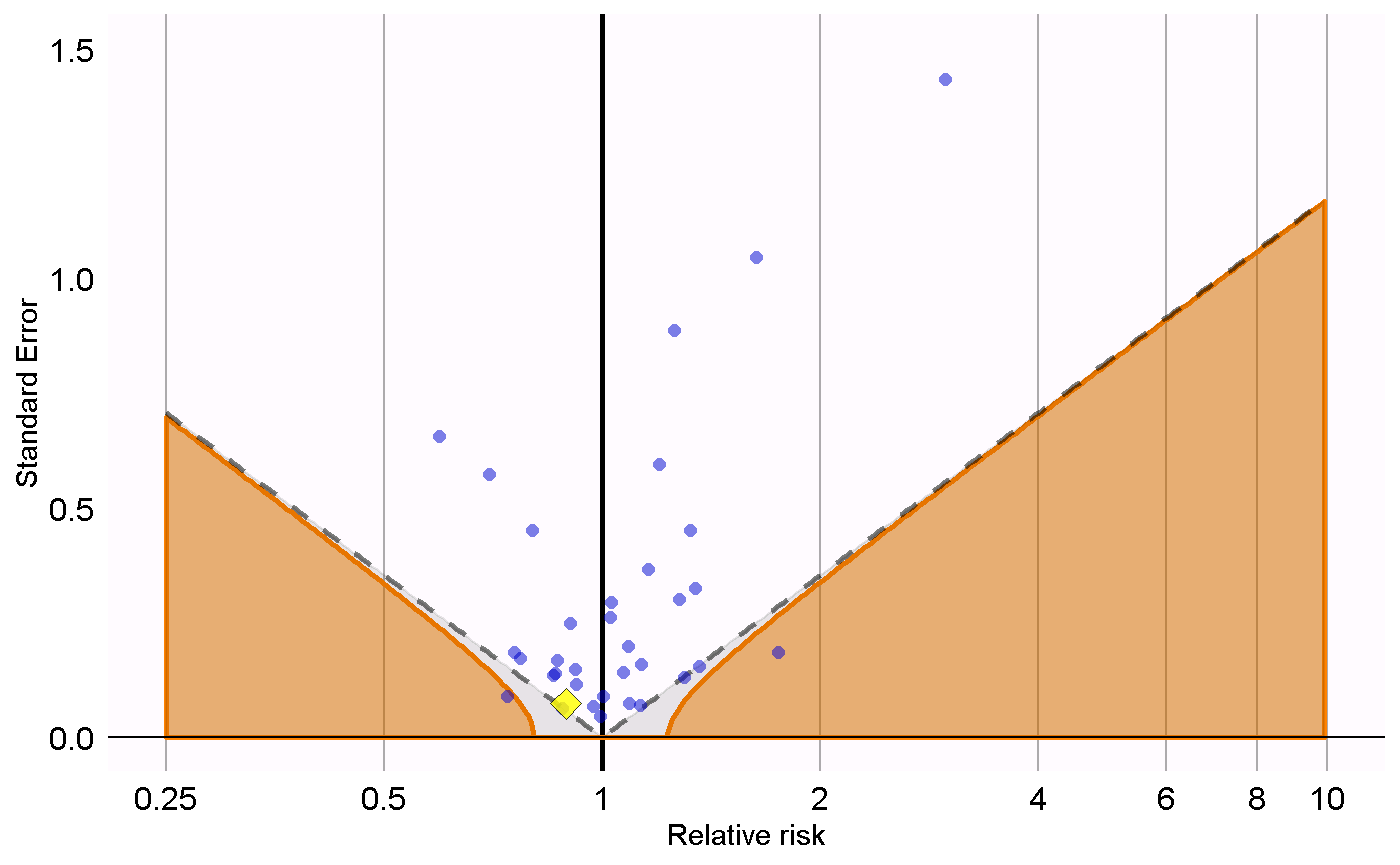
\includegraphics{../inst/doc/SingleStudies_files/figure-latex/unnamed-chunk-21-1.pdf}

It is also possible to inspect the propensity model itself by showing
the covariates that have non-zero coefficients:

\begin{Shaded}
\begin{Highlighting}[]
\NormalTok{propensityModel <-}\StringTok{ }\KeywordTok{getPsModel}\NormalTok{(ps, cohortMethodData)}
\KeywordTok{head}\NormalTok{(propensityModel)}
\end{Highlighting}
\end{Shaded}

\begin{verbatim}
#>             coefficient covariateId                               covariateName
#> (Intercept)   -1.725799          NA                                 (Intercept)
#> 27             1.437370     2007006                            index year: 2007
#> 955            1.339776  2101660504 ...s on knee joint; total knee arthroplasty
#> 2084           1.204203  4253901210 ... to index: Juvenile rheumatoid arthritis
#> 5             -1.165074        3003                            age group: 15-19
#> 28             1.000266     2008006                            index year: 2008
\end{verbatim}

One advantage of using the regularization when fitting the propensity
model is that most coefficients will shrink to zero and fall out of the
model. It is a good idea to inspect the remaining variables for anything
that should not be there, for example variations of the drugs of
interest that we forgot to exclude.

\hypertarget{using-the-propensity-score}{%
\subsection{Using the propensity
score}\label{using-the-propensity-score}}

We can use the propensity scores to trim, stratify, match, or weigh our
population. For example, one could trim to equipoise, meaning only
subjects with a preference score between 0.25 and 0.75 are kept:

\begin{Shaded}
\begin{Highlighting}[]
\NormalTok{trimmedPop <-}\StringTok{ }\KeywordTok{trimByPsToEquipoise}\NormalTok{(ps)}
\KeywordTok{plotPs}\NormalTok{(trimmedPop, ps, }\DataTypeTok{scale =} \StringTok{"preference"}\NormalTok{)}
\end{Highlighting}
\end{Shaded}

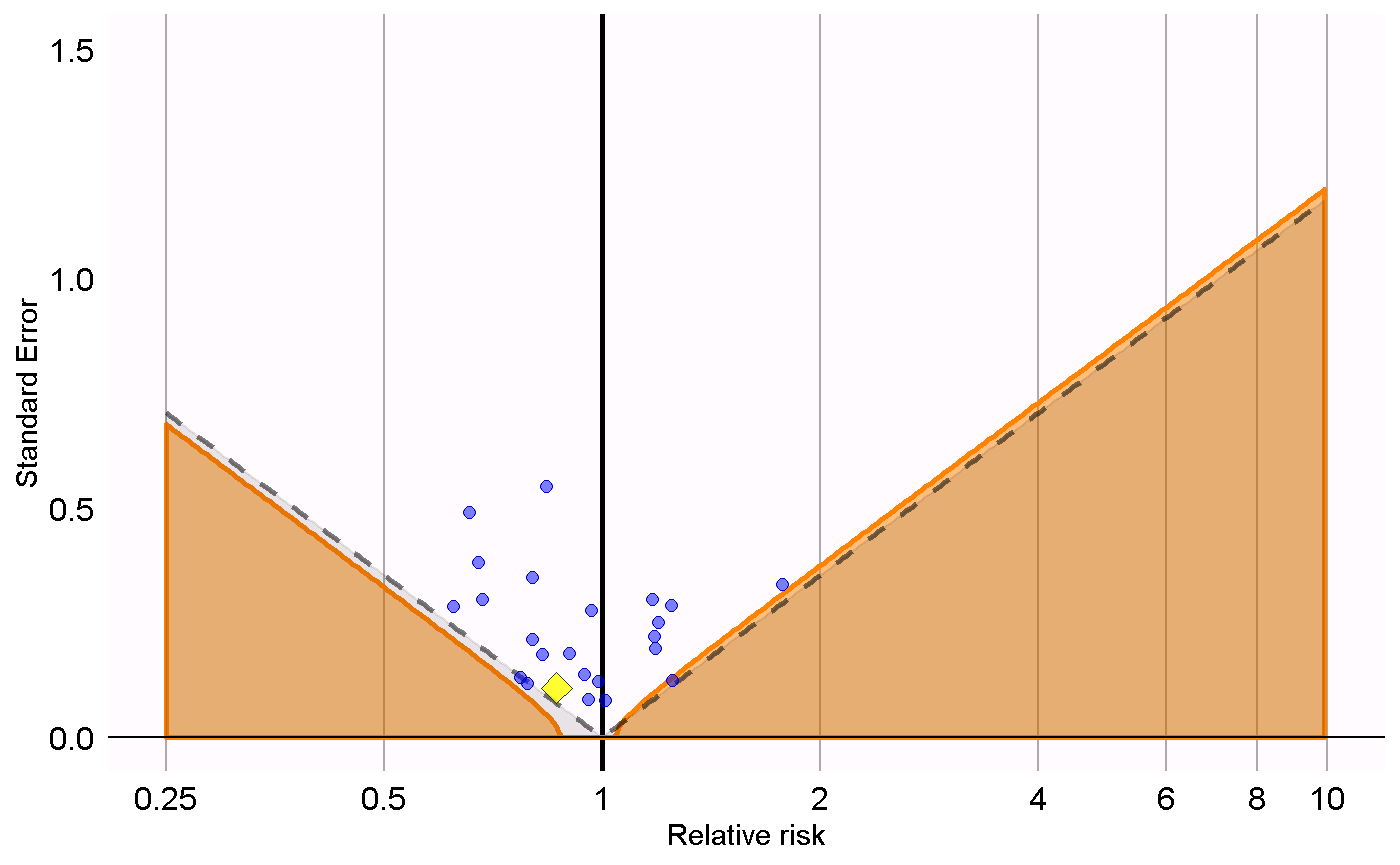
\includegraphics{../inst/doc/SingleStudies_files/figure-latex/unnamed-chunk-25-1.pdf}

Instead (or additionally), we could stratify the population based on the
propensity score:

\begin{Shaded}
\begin{Highlighting}[]
\NormalTok{stratifiedPop <-}\StringTok{ }\KeywordTok{stratifyByPs}\NormalTok{(ps, }\DataTypeTok{numberOfStrata =} \DecValTok{5}\NormalTok{)}
\KeywordTok{plotPs}\NormalTok{(stratifiedPop, ps, }\DataTypeTok{scale =} \StringTok{"preference"}\NormalTok{)}
\end{Highlighting}
\end{Shaded}

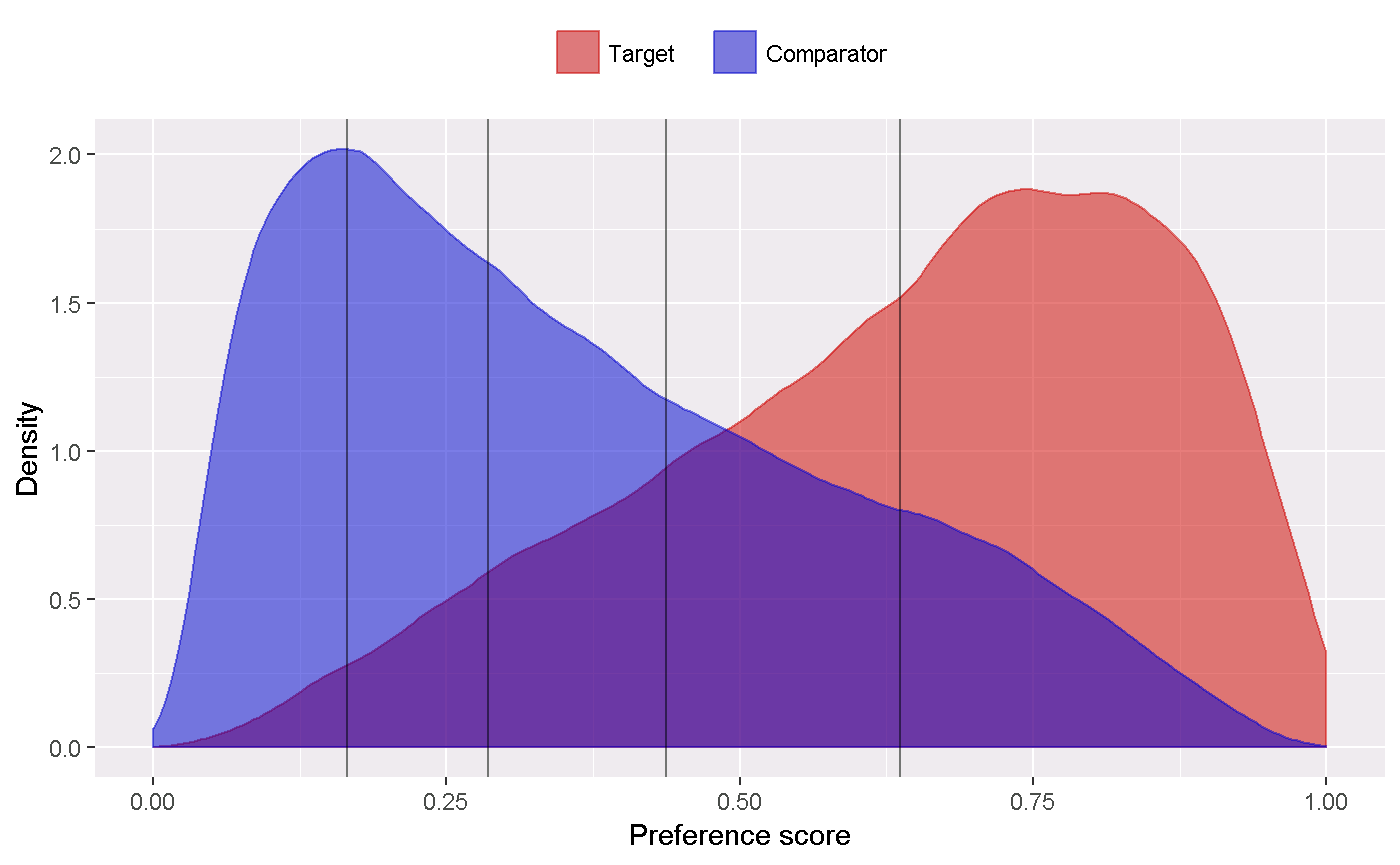
\includegraphics{../inst/doc/SingleStudies_files/figure-latex/unnamed-chunk-27-1.pdf}

We can also match subjects based on propensity scores. In this example,
we're using one-to-one matching:

\begin{Shaded}
\begin{Highlighting}[]
\NormalTok{matchedPop <-}\StringTok{ }\KeywordTok{matchOnPs}\NormalTok{(ps, }\DataTypeTok{caliper =} \FloatTok{0.2}\NormalTok{, }\DataTypeTok{caliperScale =} \StringTok{"standardized logit"}\NormalTok{, }\DataTypeTok{maxRatio =} \DecValTok{1}\NormalTok{)}
\KeywordTok{plotPs}\NormalTok{(matchedPop, ps)}
\end{Highlighting}
\end{Shaded}

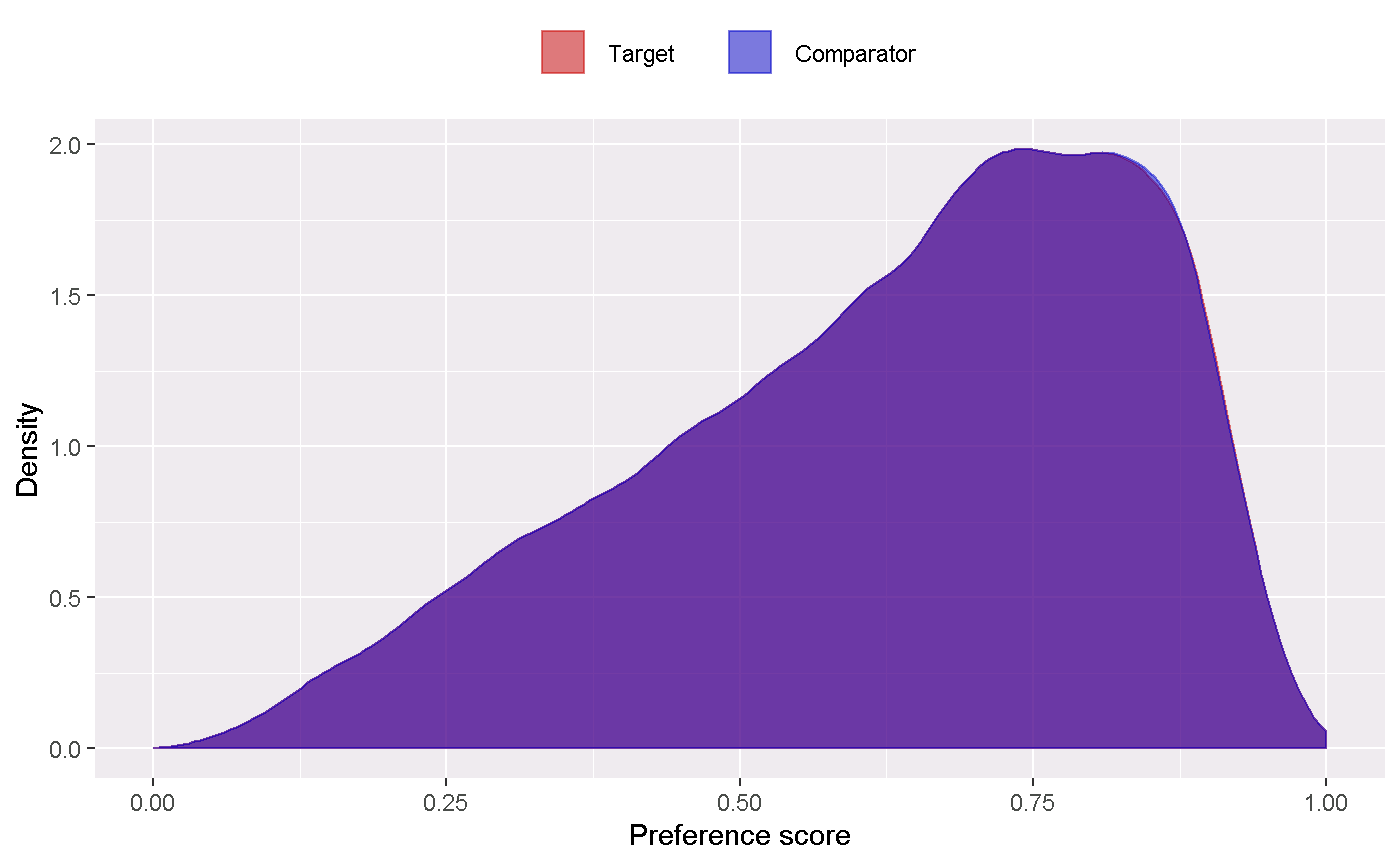
\includegraphics{../inst/doc/SingleStudies_files/figure-latex/unnamed-chunk-29-1.pdf}

Note that for both stratification and matching it is possible to specify
additional matching criteria such as age and sex using the
\texttt{stratifyByPsAndCovariates()} and
\texttt{matchOnPsAndCovariates()} functions, respectively.

We can see the effect of trimming and/or matching on the population
using the \texttt{getAttritionTable} function:

\begin{Shaded}
\begin{Highlighting}[]
\KeywordTok{getAttritionTable}\NormalTok{(matchedPop)}
\end{Highlighting}
\end{Shaded}

\begin{verbatim}
#>                                                               description targetPersons comparatorPersons targetExposures comparatorExposures
#> 1                                                        Original cohorts        104225            511194          184979              798752
#> 2 First exp. only & removed subs in both cohorts & 180 days of obs. prior         49102            348558           49102              348558
#> 3                                                        No prior outcome         47411            339992           47411              339992
#> 4                                            Have at least 1 days at risk         47377            339648           47377              339648
#> 5                                             Matched on propensity score         44901             44901           44901               44901
\end{verbatim}

Or, if we like, we can plot an attrition diagram:

\begin{Shaded}
\begin{Highlighting}[]
\KeywordTok{drawAttritionDiagram}\NormalTok{(matchedPop)}
\end{Highlighting}
\end{Shaded}

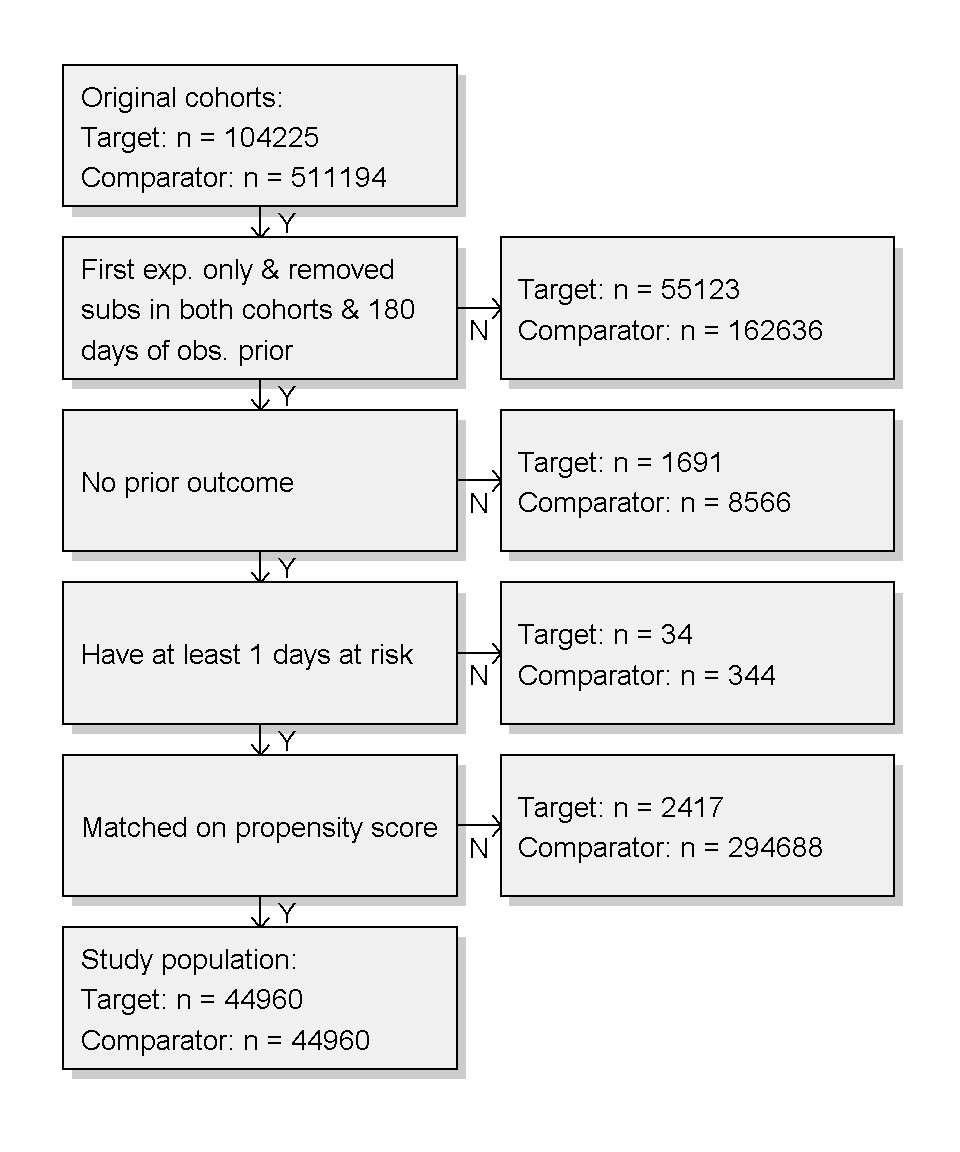
\includegraphics{../inst/doc/SingleStudies_files/figure-latex/unnamed-chunk-33-1.pdf}

\hypertarget{evaluating-covariate-balance}{%
\subsection{Evaluating covariate
balance}\label{evaluating-covariate-balance}}

To evaluate whether our use of the propensity score is indeed making the
two cohorts more comparable, we can compute the covariate balance before
and after trimming, matching, and/or stratifying:

\begin{Shaded}
\begin{Highlighting}[]
\NormalTok{balance <-}\StringTok{ }\KeywordTok{computeCovariateBalance}\NormalTok{(matchedPop, cohortMethodData)}
\end{Highlighting}
\end{Shaded}

\begin{Shaded}
\begin{Highlighting}[]
\KeywordTok{plotCovariateBalanceScatterPlot}\NormalTok{(balance, }\DataTypeTok{showCovariateCountLabel =} \OtherTok{TRUE}\NormalTok{, }\DataTypeTok{showMaxLabel =} \OtherTok{TRUE}\NormalTok{)}
\end{Highlighting}
\end{Shaded}

\begin{verbatim}
#> Warning: Removed 10591 rows containing missing values (geom_point).
\end{verbatim}

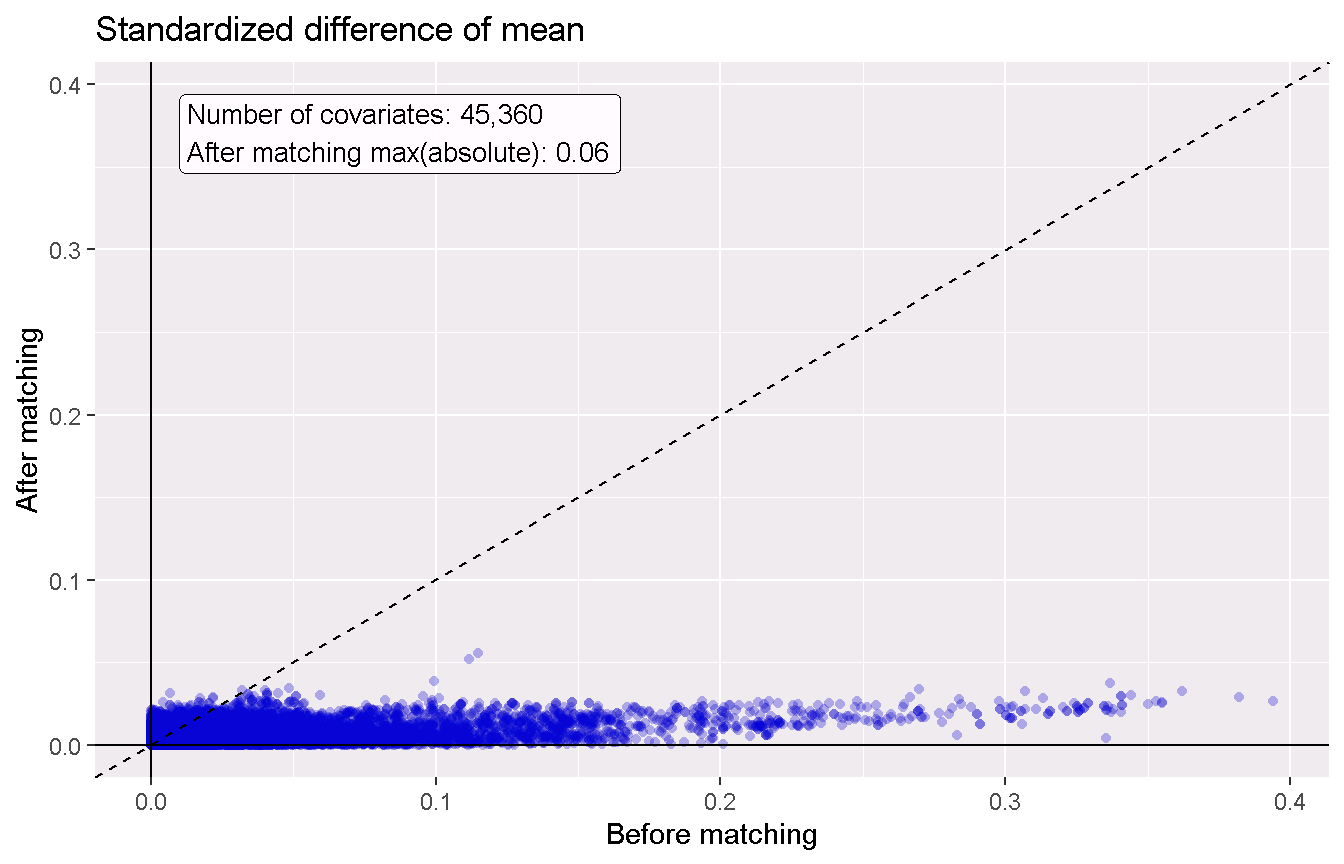
\includegraphics{../inst/doc/SingleStudies_files/figure-latex/unnamed-chunk-37-1.pdf}

\begin{Shaded}
\begin{Highlighting}[]
\KeywordTok{plotCovariateBalanceOfTopVariables}\NormalTok{(balance)}
\end{Highlighting}
\end{Shaded}

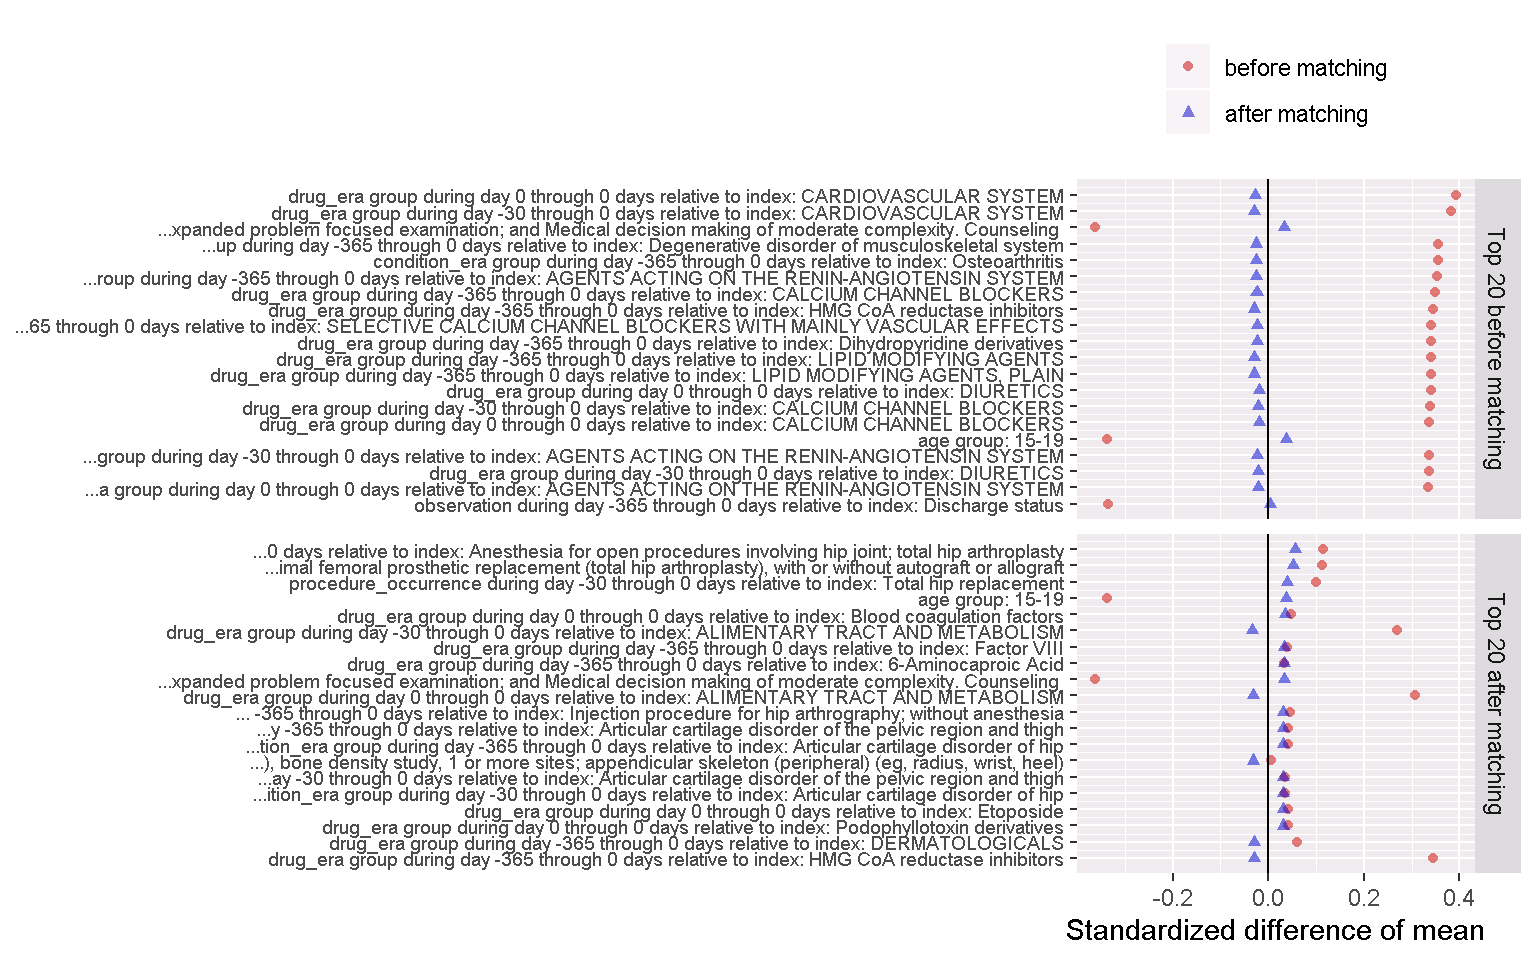
\includegraphics{../inst/doc/SingleStudies_files/figure-latex/unnamed-chunk-39-1.pdf}

The `before matching' population is the population as extracted by the
\texttt{getDbCohortMethodData} function, so before any further filtering
steps.

\hypertarget{inspecting-select-population-characteristics}{%
\subsection{Inspecting select population
characteristics}\label{inspecting-select-population-characteristics}}

It is customary to include a table in your paper that lists some select
population characteristics before and after
matching/stratification/trimming. This is usually the first table, and
so will be referred to as `table 1'. To generate this table, you can use
the \texttt{createCmTable1} function:

\begin{Shaded}
\begin{Highlighting}[]
\KeywordTok{createCmTable1}\NormalTok{(balance)}
\end{Highlighting}
\end{Shaded}

\fontsize{6.5}{6.5}
\selectfont

\begin{verbatim}
                                                         Before matching                      After matching                     
                                                         Target          Comparator           Target         Comparator          
 Characteristic                                          %               %          Std. diff %              %          Std. diff
 Age group                                                                                                                       
   00-04                                                  0.1             0.1        0.02      0.1            0.0        0.02    
   05-09                                                  0.3             0.2        0.02      0.2            0.2        0.00    
   10-14                                                  0.8             2.3       -0.12      0.8            0.7        0.02    
   15-19                                                  2.7            11.1       -0.34      2.8            2.3        0.04    
   20-24                                                  2.2             6.5       -0.21      2.3            2.0        0.02    
   25-29                                                  3.9             9.6       -0.23      4.1            3.7        0.02    
   30-34                                                  5.7            11.0       -0.19      6.0            5.7        0.01    
   35-39                                                  7.0            10.8       -0.14      7.2            7.1        0.00    
   40-44                                                  9.0             9.7       -0.02      9.2            9.3        0.00    
   45-49                                                 11.1             9.4        0.06     11.2           11.6       -0.01    
   50-54                                                 13.6             9.7        0.12     13.4           13.8       -0.01    
   55-59                                                 13.3             8.5        0.16     13.3           13.7       -0.01    
   60-64                                                 12.0             5.6        0.23     11.6           12.1       -0.01    
   65-69                                                  5.5             1.8        0.20      5.2            5.2        0.00    
   70-74                                                  4.2             1.2        0.18      4.0            4.0        0.00    
   75-79                                                  3.4             1.0        0.16      3.3            3.3        0.00    
   80-84                                                  2.9             0.8        0.16      2.8            2.8        0.00    
   85-89                                                  2.2             0.7        0.13      2.1            2.2       -0.01    
   90-94                                                  0.1             0.1        0.02      0.1            0.1        0.01    
 Gender: female                                          69.6            71.9       -0.05     69.9           70.0        0.00    
 Race                                                                                                                            
   race = Black or African American                      17.7            27.5       -0.24     17.9           17.0        0.02    
   race = Other Race                                     20.1            17.8        0.06     20.8           21.5       -0.02    
   race = White                                          62.2            54.7        0.15     61.3           61.4        0.00    
 Ethnicity                                                                                                                       
   ethnicity = Hispanic or Latino                         1.6             2.2       -0.04      1.7            1.7        0.00    
   ethnicity = Not Hispanic or Latino                    18.4            15.7        0.07     19.1           19.8       -0.02    
 Medical history: General                                                                                                        
   Acute respiratory disease                             31.0            34.5       -0.08     30.3           29.8        0.01    
   Attention deficit hyperactivity disorder               2.1             3.8       -0.10      2.1            2.0        0.01    
   Chronic liver disease                                  4.4             3.2        0.06      4.1            4.3       -0.01    
   Chronic obstructive lung disease                      16.5             9.3        0.22     15.3           15.5       -0.01    
   Crohn's disease                                        0.6             0.4        0.03      0.5            0.5        0.00    
   Dementia                                               2.0             0.8        0.10      1.7            1.7        0.00    
   Depressive disorder                                   30.0            26.3        0.08     28.8           29.2       -0.01    
   Diabetes mellitus                                     22.6            15.1        0.19     21.7           22.3       -0.01    
   Gastroesophageal reflux disease                       21.8            16.4        0.14     20.4           20.9       -0.01    
   Gastrointestinal hemorrhage                            3.9             2.8        0.06      2.1            2.1       -0.01    
   Human immunodeficiency virus infection                 0.6             0.7       -0.01      0.6            0.6        0.00    
   Hyperlipidemia                                        31.4            21.9        0.22     30.6           31.8       -0.03    
   Hypertensive disorder                                 45.7            33.3        0.26     44.0           44.7       -0.01    
   Lesion of liver                                        1.3             0.8        0.04      1.0            1.1        0.00    
   Obesity                                               14.9            14.9        0.00     14.4           14.6       -0.01    
   Osteoarthritis                                        38.7            22.6        0.36     36.6           37.8       -0.03    
   Pneumonia                                              5.4             3.4        0.10      4.8            4.8        0.00    
   Psoriasis                                              1.0             0.7        0.03      1.0            1.0        0.00    
   Renal impairment                                       4.5             3.0        0.08      3.9            4.1       -0.01    
   Rheumatoid arthritis                                   4.1             2.0        0.13      3.8            4.1       -0.02    
   Schizophrenia                                          3.0             2.1        0.06      2.6            2.6        0.00    
   Ulcerative colitis                                     0.4             0.2        0.03      0.3            0.3       -0.01    
   Urinary tract infectious disease                      13.2            14.5       -0.04     12.4           12.6        0.00    
   Viral hepatitis C                                      3.2             2.4        0.05      3.0            3.2       -0.01    
   Visual system disorder                                31.6            27.6        0.09     30.7           31.0       -0.01    
 Medical history: Cardiovascular disease                                                                                         
   Atrial fibrillation                                    2.5             1.1        0.11      2.2            2.4       -0.02    
   Cerebrovascular disease                                5.1             3.1        0.10      4.6            4.7        0.00    
   Coronary arteriosclerosis                              8.9             4.5        0.18      8.1            8.5       -0.02    
   Heart disease                                         23.7            14.2        0.25     21.7           22.3       -0.01    
   Heart failure                                          6.2             3.3        0.14      5.5            5.6       -0.01    
   Ischemic heart disease                                 6.3             3.4        0.13      5.7            5.9       -0.01    
   Peripheral vascular disease                           11.9             6.4        0.19     10.8           11.3       -0.02    
   Pulmonary embolism                                     1.1             0.5        0.07      0.9            0.9       -0.01    
   Venous thrombosis                                      3.0             1.6        0.09      2.6            2.6        0.00    
 Medical history: Neoplasms                                                                                                      
   Hematologic neoplasm                                   1.2             0.5        0.07      1.0            1.0        0.00    
   Malignant lymphoma                                     0.4             0.2        0.03      0.3            0.3        0.00    
   Malignant neoplasm of anorectum                        0.2             0.1        0.04      0.2            0.2        0.00    
   Malignant neoplastic disease                           6.3             3.2        0.15      5.6            5.7        0.00    
   Malignant tumor of breast                              1.5             0.8        0.06      1.4            1.6       -0.01    
   Malignant tumor of colon                               0.4             0.2        0.04      0.3            0.3        0.00    
   Malignant tumor of lung                                0.5             0.1        0.06      0.4            0.4        0.00    
   Malignant tumor of urinary bladder                     0.2             0.1        0.03      0.2            0.1        0.00    
   Primary malignant neoplasm of prostate                 0.4             0.2        0.04      0.3            0.3        0.00    
 Medication use                                                                                                                  
   Agents acting on the renin-angiotensin system         49.5            32.4        0.35     48.4           49.7       -0.03    
   Antibacterials for systemic use                       72.3            72.9       -0.01     71.5           72.1       -0.01    
   Antidepressants                                       61.2            51.0        0.21     59.8           61.0       -0.02    
   Antiepileptics                                        73.7            72.0        0.04     72.9           73.8       -0.02    
   Antiinflammatory and antirheumatic products            0.0             0.0        0.01      0.0            0.0        0.00    
   Antineoplastic agents                                 17.7            14.7        0.08     16.3           16.4        0.00    
   Antipsoriatics                                         7.7             6.7        0.04      7.7            8.1       -0.02    
   Antithrombotic agents                                 20.5             9.7        0.31     18.2           19.0       -0.02    
   Beta blocking agents                                  50.9            36.6        0.29     49.6           50.5       -0.02    
   Calcium channel blockers                              51.0            34.0        0.35     50.1           51.3       -0.02    
   Diuretics                                             59.8            44.4        0.31     58.6           59.6       -0.02    
   Drugs for acid related disorders                      69.1            64.0        0.11     67.9           69.1       -0.03    
   Drugs for obstructive airway diseases                 56.5            55.1        0.03     55.7           56.4       -0.01    
   Drugs used in diabetes                                29.6            19.0        0.25     28.9           29.9       -0.02    
   Immunosuppressants                                     3.4             1.7        0.11      3.2            3.5       -0.02    
   Lipid modifying agents                                42.3            26.4        0.34     41.3           42.8       -0.03    
   Opioids                                               73.5            73.5        0.00     72.6           73.2       -0.01    
   Psycholeptics                                         82.3            78.2        0.10     81.5           82.2       -0.02    
   Psychostimulants, agents used for adhd and nootropics 69.9            70.6       -0.02     69.0           69.6       -0.01    
\end{verbatim}

\fontsize{10}{12}
\selectfont

\hypertarget{inserting-the-population-cohort-in-the-database}{%
\subsection{Inserting the population cohort in the
database}\label{inserting-the-population-cohort-in-the-database}}

For various reasons it might be necessary to insert the study population
back into the database, for example because we want to use an external
cohort characterization tool. We can use the \texttt{insertDbPopulation}
function for this purpose:

\begin{Shaded}
\begin{Highlighting}[]
\KeywordTok{insertDbPopulation}\NormalTok{(}\DataTypeTok{population =}\NormalTok{ matchedPop,}
                   \DataTypeTok{cohortIds =} \KeywordTok{c}\NormalTok{(}\DecValTok{101}\NormalTok{,}\DecValTok{100}\NormalTok{),}
                   \DataTypeTok{connectionDetails =}\NormalTok{ connectionDetails,}
                   \DataTypeTok{cohortDatabaseSchema =}\NormalTok{ resultsDatabaseSchema,}
                   \DataTypeTok{cohortTable =} \StringTok{"coxibVsNonselVsGiBleed"}\NormalTok{,}
                   \DataTypeTok{createTable =} \OtherTok{FALSE}\NormalTok{,}
                   \DataTypeTok{cdmVersion =}\NormalTok{ cdmVersion)}
\end{Highlighting}
\end{Shaded}

This function will store the population in a table with the same
structure as the \texttt{cohort} table in the CDM, in this case in the
same table where we had created our original cohorts.

\hypertarget{follow-up-and-power}{%
\section{Follow-up and power}\label{follow-up-and-power}}

Before we start fitting an outcome model, we might be interested to know
whether we have sufficient power to detect a particular effect size. It
makes sense to perform these power calculations once the study
population has been fully defined, so taking into account loss to the
various inclusion and exclusion criteria (such as no prior outcomes),
and loss due to matching and/or trimming. Since the sample size is fixed
in retrospective studies (the data has already been collected), and the
true effect size is unknown, the CohortMethod package provides a
function to compute the minimum detectable relative risk (MDRR) instead:

\begin{Shaded}
\begin{Highlighting}[]
\KeywordTok{computeMdrr}\NormalTok{(}\DataTypeTok{population =}\NormalTok{ studyPop,}
            \DataTypeTok{modelType =} \StringTok{"cox"}\NormalTok{,}
            \DataTypeTok{alpha =} \FloatTok{0.05}\NormalTok{,}
            \DataTypeTok{power =} \FloatTok{0.8}\NormalTok{,}
            \DataTypeTok{twoSided =} \OtherTok{TRUE}\NormalTok{)}
\end{Highlighting}
\end{Shaded}

\fontsize{6.5}{6.5}
\selectfont

\begin{verbatim}
#>   targetPersons comparatorPersons targetExposures comparatorExposures targetDays comparatorDays totalOutcomes     mdrr         se
#> 1         47377            339648           47377              339648    6609395       23763641          1215 1.277903 0.08752912
\end{verbatim}

\fontsize{10}{12}
\selectfont

In this example we used the \texttt{studyPop} object, so the population
before any matching or trimming. If we want to know the MDRR after
matching, we use the \texttt{matchedPop} object we created earlier
instead:

\begin{Shaded}
\begin{Highlighting}[]
\KeywordTok{computeMdrr}\NormalTok{(}\DataTypeTok{population =}\NormalTok{ matchedPop,}
            \DataTypeTok{modelType =} \StringTok{"cox"}\NormalTok{,}
            \DataTypeTok{alpha =} \FloatTok{0.05}\NormalTok{,}
            \DataTypeTok{power =} \FloatTok{0.8}\NormalTok{,}
            \DataTypeTok{twoSided =} \OtherTok{TRUE}\NormalTok{)}
\end{Highlighting}
\end{Shaded}

\fontsize{6.5}{6.5}
\selectfont

\begin{verbatim}
#>   targetPersons comparatorPersons targetExposures comparatorExposures targetDays comparatorDays totalOutcomes     mdrr        se
#> 1         44901             44901           44901               44901    6196468        3929370           442 1.305408 0.0951303
\end{verbatim}

\fontsize{10}{12}
\selectfont

Even thought the MDRR in the matched population is higher, meaning we
have less power, we should of course not be fooled: matching most likely
eliminates confounding, and is therefore preferred to not matching.

To gain a better understanding of the amount of follow-up available we
can also inspect the distribution of follow-up time. We defined
follow-up time as time at risk, so not censored by the occurrence of the
outcome. The \texttt{getFollowUpDistribution} can provide a simple
overview:

\begin{Shaded}
\begin{Highlighting}[]
\KeywordTok{getFollowUpDistribution}\NormalTok{(}\DataTypeTok{population =}\NormalTok{ matchedPop)}
\end{Highlighting}
\end{Shaded}

\begin{verbatim}
#>   100% 75% 50% 25%   0% Treatment
#> 1    2  61  61 137 3764         1
#> 2    2  46  61  84 3026         0
\end{verbatim}

The output is telling us number of days of follow-up each quantile of
the study population has. We can also plot the distribution:

\begin{Shaded}
\begin{Highlighting}[]
\KeywordTok{plotFollowUpDistribution}\NormalTok{(}\DataTypeTok{population =}\NormalTok{ matchedPop)}
\end{Highlighting}
\end{Shaded}

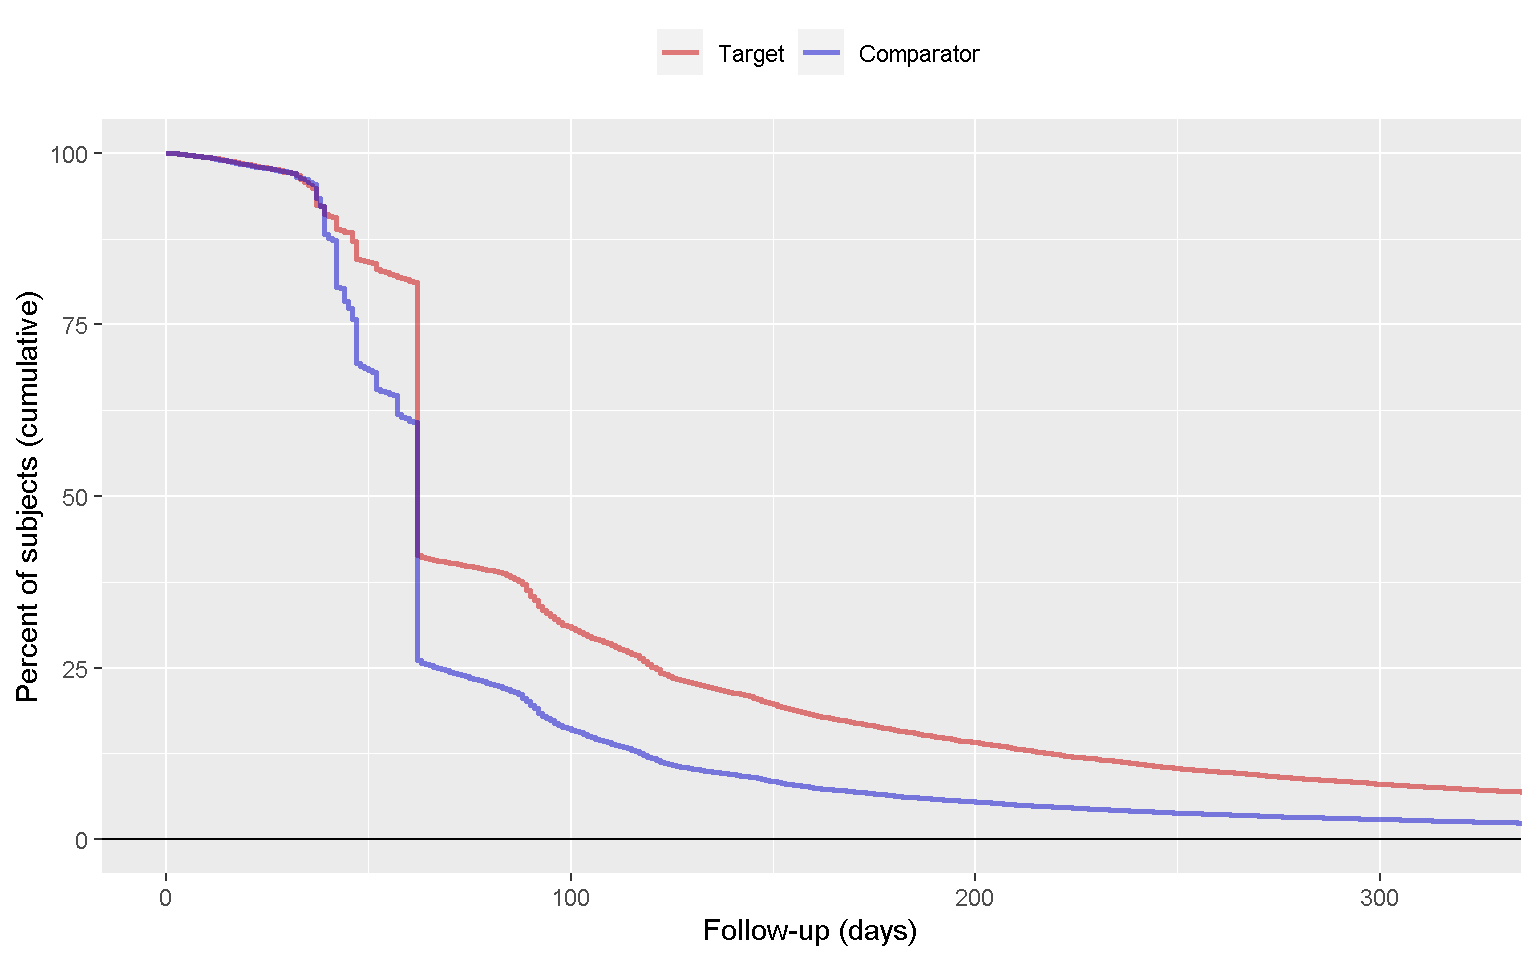
\includegraphics{../inst/doc/SingleStudies_files/figure-latex/unnamed-chunk-50-1.pdf}

\hypertarget{outcome-models}{%
\section{Outcome models}\label{outcome-models}}

The outcome model is a model describing which variables are associated
with the outcome.

\hypertarget{fitting-a-simple-outcome-model}{%
\subsection{Fitting a simple outcome
model}\label{fitting-a-simple-outcome-model}}

In theory we could fit an outcome model without using the propensity
scores. In this example we are fitting an outcome model using a Cox
regression:

\begin{Shaded}
\begin{Highlighting}[]
\NormalTok{outcomeModel <-}\StringTok{ }\KeywordTok{fitOutcomeModel}\NormalTok{(}\DataTypeTok{population =}\NormalTok{ studyPop,}
                                \DataTypeTok{modelType =} \StringTok{"cox"}\NormalTok{)}
\NormalTok{outcomeModel}
\end{Highlighting}
\end{Shaded}

\begin{verbatim}
#> Model type: cox
#> Stratified: FALSE
#> Use covariates: FALSE
#> Use inverse probability of treatment weighting: 
#> Status: OK
#> 
#>           Estimate lower .95 upper .95    logRr seLogRr
#> treatment 1.038993  0.899015  1.196863 0.038252   0.073
\end{verbatim}

But of course we want to make use of the matching done on the propensity
score:

\begin{Shaded}
\begin{Highlighting}[]
\NormalTok{outcomeModel <-}\StringTok{ }\KeywordTok{fitOutcomeModel}\NormalTok{(}\DataTypeTok{population =}\NormalTok{ matchedPop,}
                                \DataTypeTok{modelType =} \StringTok{"cox"}\NormalTok{,}
                                \DataTypeTok{stratified =} \OtherTok{TRUE}\NormalTok{)}
\NormalTok{outcomeModel}
\end{Highlighting}
\end{Shaded}

\begin{verbatim}
#> Model type: cox
#> Stratified: TRUE
#> Use covariates: FALSE
#> Use inverse probability of treatment weighting: 
#> Status: OK
#> 
#>           Estimate lower .95 upper .95    logRr seLogRr
#> treatment  0.80292   0.62382   1.03105 -0.21950  0.1282
\end{verbatim}

Note that we define the sub-population to be only those in the
\texttt{matchedPop} object, which we created earlier by matching on the
propensity score. We also now use a stratified Cox model, conditioning
on the propensity score match sets.

Instead of matching or stratifying we can also perform Inverse
Probability of Treatment Weighting (IPTW):

\begin{Shaded}
\begin{Highlighting}[]
\NormalTok{outcomeModel <-}\StringTok{ }\KeywordTok{fitOutcomeModel}\NormalTok{(}\DataTypeTok{population =}\NormalTok{ ps,}
                                \DataTypeTok{modelType =} \StringTok{"cox"}\NormalTok{,}
                                \DataTypeTok{inversePsWeighting =} \OtherTok{TRUE}\NormalTok{)}
\NormalTok{outcomeModel}
\end{Highlighting}
\end{Shaded}

\begin{verbatim}
#> Model type: cox
#> Stratified: FALSE
#> Use covariates: FALSE
#> Use inverse probability of treatment weighting: 
#> Status: OK
#> 
#>           Estimate lower .95 upper .95    logRr seLogRr
#> treatment  0.84688   0.78180   0.91747 -0.16619  0.0408
\end{verbatim}

\hypertarget{adding-interaction-terms}{%
\subsection{Adding interaction terms}\label{adding-interaction-terms}}

We may be interested whether the effect is different across different
groups in the population. To explore this, we may include interaction
terms in the model. In this example we include three interaction terms:

\fontsize{5.5}{5.5}
\selectfont

\begin{Shaded}
\begin{Highlighting}[]
\NormalTok{interactionCovariateIds <-}\StringTok{ }\KeywordTok{c}\NormalTok{(}\DecValTok{8532001}\NormalTok{, }\DecValTok{201826210}\NormalTok{, }\DecValTok{21600960413}\NormalTok{) }
\CommentTok{# 8532001 = Female}
\CommentTok{# 201826210 = Type 2 Diabetes}
\CommentTok{# 21600960413 = Concurent use of antithrombotic agents}
\NormalTok{outcomeModel <-}\StringTok{ }\KeywordTok{fitOutcomeModel}\NormalTok{(}\DataTypeTok{population =}\NormalTok{ matchedPop,}
                                \DataTypeTok{modelType =} \StringTok{"cox"}\NormalTok{,}
                                \DataTypeTok{stratified =} \OtherTok{TRUE}\NormalTok{,}
                                \DataTypeTok{interactionCovariateIds =}\NormalTok{ interactionCovariateIds)}
\NormalTok{outcomeModel}
\end{Highlighting}
\end{Shaded}

\begin{verbatim}
#> Model type: cox
#> Stratified: TRUE
#> Use covariates: FALSE
#> Use inverse probability of treatment weighting: 
#> Status: OK
#> 
#>                                                                                                            Estimate lower .95 upper .95    logRr seLogRr
#> treatment                                                                                                   0.65598   0.33898   1.25086 -0.42163  0.3331
#> treatment * gender = FEMALE                                                                                 1.36524   0.61425   3.06761  0.31133  0.4103
#> treatment * drug_era group during day 0 through 0 days relative to index: ANTITHROMBOTIC AGENTS             1.19888   0.52095   2.76784  0.18139  0.4261
#> treatment * condition_era group during day -365 through 0 days relative to index: Type 2 diabetes mellitus  0.64418   0.24215   1.65443 -0.43978  0.4902
\end{verbatim}

\fontsize{10}{12}
\selectfont

Note that you can use the \texttt{grepCovariateNames} to find covariate
IDs.

It is prudent to verify that covariate balance has also been achieved in
the subgroups of interest. For example, we can check the covariate
balance in the subpopulation of females:

\begin{Shaded}
\begin{Highlighting}[]
\NormalTok{balanceFemale <-}\StringTok{ }\KeywordTok{computeCovariateBalance}\NormalTok{(}\DataTypeTok{population =}\NormalTok{ matchedPop, }
                                         \DataTypeTok{cohortMethodData =}\NormalTok{ cohortMethodData, }
                                         \DataTypeTok{subgroupCovariateId =} \DecValTok{8532001}\NormalTok{)}
\KeywordTok{plotCovariateBalanceScatterPlot}\NormalTok{(balanceFemale)}
\end{Highlighting}
\end{Shaded}

\begin{verbatim}
#> Warning: Removed 10364 rows containing missing values (geom_point).
\end{verbatim}

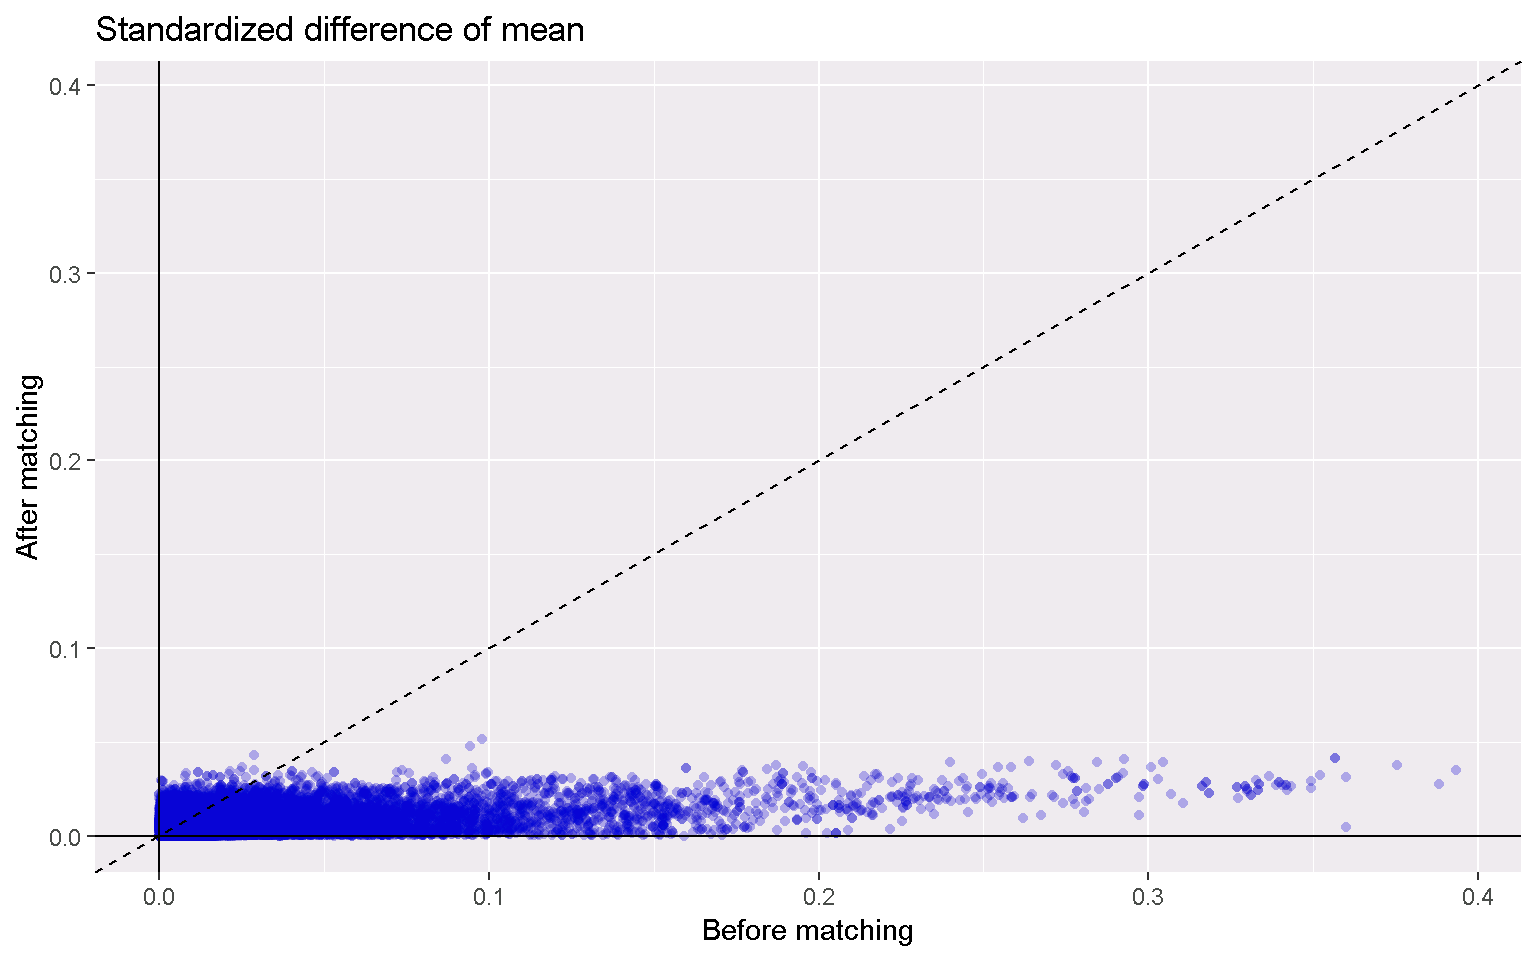
\includegraphics{../inst/doc/SingleStudies_files/figure-latex/unnamed-chunk-60-1.pdf}

\hypertarget{adding-covariates-to-the-outcome-model}{%
\subsection{Adding covariates to the outcome
model}\label{adding-covariates-to-the-outcome-model}}

One final refinement would be to use the same covariates we used to fit
the propensity model to also fit the outcome model. This way we are more
robust against misspecification of the model, and more likely to remove
bias. For this we use the regularized Cox regression in the
\texttt{Cyclops} package. (Note that the treatment variable is
automatically excluded from regularization.)

\begin{Shaded}
\begin{Highlighting}[]
\NormalTok{outcomeModel <-}\StringTok{ }\KeywordTok{fitOutcomeModel}\NormalTok{(}\DataTypeTok{population =}\NormalTok{ matchedPop,}
                                \DataTypeTok{cohortMethodData =}\NormalTok{ cohortMethodData,}
                                \DataTypeTok{modelType =} \StringTok{"cox"}\NormalTok{,}
                                \DataTypeTok{stratified =} \OtherTok{TRUE}\NormalTok{,}
                                \DataTypeTok{useCovariates =} \OtherTok{TRUE}\NormalTok{)}
\NormalTok{outcomeModel}
\end{Highlighting}
\end{Shaded}

\begin{verbatim}
#> Model type: cox
#> Stratified: TRUE
#> Use covariates: TRUE
#> Use inverse probability of treatment weighting: 
#> Status: OK
#> Prior variance: 0.0417214627426502
#> 
#>           Estimate lower .95 upper .95    logRr seLogRr
#> treatment  0.85190   0.63285   1.14949 -0.16029  0.1523
\end{verbatim}

\hypertarget{inpecting-the-outcome-model}{%
\subsection{Inpecting the outcome
model}\label{inpecting-the-outcome-model}}

We can inspect more details of the outcome model:

\begin{Shaded}
\begin{Highlighting}[]
\KeywordTok{summary}\NormalTok{(outcomeModel)}
\end{Highlighting}
\end{Shaded}

\begin{verbatim}
#> Model type: cox
#> Stratified: TRUE
#> Use covariates: TRUE
#> Use inverse probability of treatment weighting: 
#> Status: OK
#> Prior variance: 0.0417214627426502
#> 
#>           Estimate lower .95 upper .95    logRr seLogRr
#> treatment  0.85190   0.63285   1.14949 -0.16029  0.1523
#> 
#> Population counts
#>       treatedPersons comparatorPersons treatedExposures comparatorExposures
#> Count          44840             44840            44840               44840
#> 
#> Outcome counts
#>       treatedPersons comparatorPersons treatedExposures comparatorExposures treatedOutcomes
#> Count            245               196              245                 196             245
#> 
#> Time at risk
#>      treatedDays comparatorDays
#> Days     6144026        3904722
\end{verbatim}

\begin{Shaded}
\begin{Highlighting}[]
\KeywordTok{exp}\NormalTok{(}\KeywordTok{coef}\NormalTok{(outcomeModel))}
\end{Highlighting}
\end{Shaded}

\begin{verbatim}
#> [1] 0.8518951
\end{verbatim}

\begin{Shaded}
\begin{Highlighting}[]
\KeywordTok{exp}\NormalTok{(}\KeywordTok{confint}\NormalTok{(outcomeModel))}
\end{Highlighting}
\end{Shaded}

\begin{verbatim}
#> [1] 0.6328451 1.1494942
\end{verbatim}

We can also see the covariates that ended up in the outcome model:

\begin{Shaded}
\begin{Highlighting}[]
\NormalTok{fullOutcomeModel <-}\StringTok{ }\KeywordTok{getOutcomeModel}\NormalTok{(outcomeModel, cohortMethodData)}
\KeywordTok{head}\NormalTok{(fullOutcomeModel)}
\end{Highlighting}
\end{Shaded}

\begin{verbatim}
#>             coefficient          id                               covariateName
#> 198124210     0.5499190   198124210 ...0 days relative to index: Kidney disease
#> 8507001       0.4828838     8507001                               gender = MALE
#> 2514408502    0.3252432  2514408502 ...nation; Medical decision making of moder
#> 21601664412   0.3017819 21601664412 ... relative to index: BETA BLOCKING AGENTS
#> 4329041212    0.2805469  4329041212 ...0 through 0 days relative to index: Pain
#> 321588210     0.2762147   321588210 ... 0 days relative to index: Heart disease
\end{verbatim}

\hypertarget{kaplan-meier-plot}{%
\subsection{Kaplan-Meier plot}\label{kaplan-meier-plot}}

We can create the Kaplan-Meier plot:

\begin{Shaded}
\begin{Highlighting}[]
\KeywordTok{plotKaplanMeier}\NormalTok{(matchedPop, }\DataTypeTok{includeZero =} \OtherTok{FALSE}\NormalTok{)}
\end{Highlighting}
\end{Shaded}

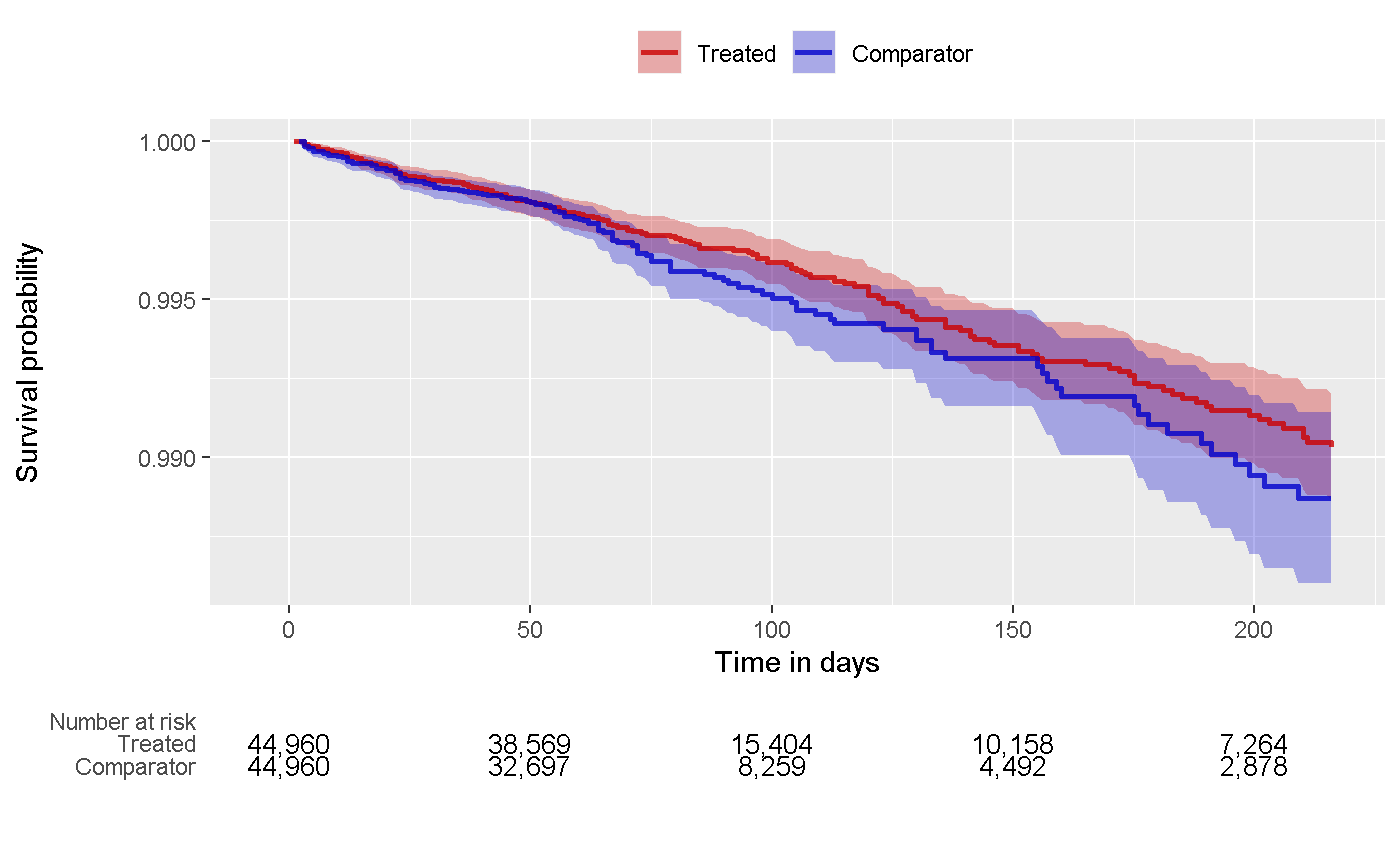
\includegraphics{../inst/doc/SingleStudies_files/figure-latex/unnamed-chunk-72-1.pdf}

Note that the Kaplan-Meier plot will automatically adjust for any
stratification, matching, or trimming that may have been applied.

\hypertarget{acknowledgments}{%
\section{Acknowledgments}\label{acknowledgments}}

Considerable work has been dedicated to provide the
\texttt{CohortMethod} package.

\begin{Shaded}
\begin{Highlighting}[]
\KeywordTok{citation}\NormalTok{(}\StringTok{"CohortMethod"}\NormalTok{)}
\end{Highlighting}
\end{Shaded}

\begin{verbatim}
#> 
#> To cite package 'CohortMethod' in publications use:
#> 
#>   Martijn J. Schuemie, Marc A. Suchard and Patrick B. Ryan (2018). CohortMethod: New-user cohort method with large scale propensity and outcome models. R package version 3.0.0.
#> 
#> A BibTeX entry for LaTeX users is
#> 
#>   @Manual{,
#>     title = {CohortMethod: New-user cohort method with large scale propensity and outcome models},
#>     author = {Martijn J. Schuemie and Marc A. Suchard and Patrick B. Ryan},
#>     year = {2018},
#>     note = {R package version 3.0.0},
#>   }
#> 
#> ATTENTION: This citation information has been auto-generated from the package DESCRIPTION file and may need manual editing, see 'help("citation")'.
\end{verbatim}

Further, \texttt{CohortMethod} makes extensive use of the
\texttt{Cyclops} package.

\begin{Shaded}
\begin{Highlighting}[]
\KeywordTok{citation}\NormalTok{(}\StringTok{"Cyclops"}\NormalTok{)}
\end{Highlighting}
\end{Shaded}

\begin{verbatim}
#> 
#> To cite Cyclops in publications use:
#> 
#> Suchard MA, Simpson SE, Zorych I, Ryan P and Madigan D (2013). "Massive parallelization of serial inference algorithms for complex generalized linear models." _ACM Transactions on
#> Modeling and Computer Simulation_, *23*, pp. 10. <URL: http://dl.acm.org/citation.cfm?id=2414791>.
#> 
#> A BibTeX entry for LaTeX users is
#> 
#>   @Article{,
#>     author = {M. A. Suchard and S. E. Simpson and I. Zorych and P. Ryan and D. Madigan},
#>     title = {Massive parallelization of serial inference algorithms for complex generalized linear models},
#>     journal = {ACM Transactions on Modeling and Computer Simulation},
#>     volume = {23},
#>     pages = {10},
#>     year = {2013},
#>     url = {http://dl.acm.org/citation.cfm?id=2414791},
#>   }
\end{verbatim}

This work is supported in part through the National Science Foundation
grant IIS 1251151.


\end{document}
